\documentclass[10pt]{article}
\usepackage{graphicx}
\usepackage{amsmath}
\usepackage{amssymb}

\begin{document}

\newcommand{\josquote}[1]{
    \framebox{
    \parbox{\textwidth}{
    \textit{#1}
    }
    }
}

\newcommand{\paulhint}[1]{
    #1
}

\setlength\parindent{0pt}
\section{Linearity and Time Invariance; Time-Domain Representations}
%
\subsection*{Linearity and Time Invariance; Time-Domain Representations}

$ y_n = b_0 x_n + b_1 x_n +  \cdots + b_Mx_{n*m}
    - a_1 y_{n-1} \cdots -a_n y_{n-N}$

\subsection*{Recall the simplest lowpass filter}
$ y_n = x_n + x_{n - 1} 
\\
            (M=1, N =0) \\
            (b_0 = 1, b_1 = 1)$

(FIR, order 1) 

$h_n = \delta_n + \delta_{n - 1} = [1, 1, 0, \dots]$\\

freq response:\\
$H(w) = \mbox{DTFT}(h) = 1 + e^{-jwT}$\\
phase response:\\
$\Theta(w) = \angle H(w) = -wt/2  = -\pi f T$ \\
phase delay: \\
$P(\omega) = -\theta(\omega)/N = + T / 2$ \\
group delay: \\
    $D(\omega) = -2 / ??? \theta(\omega) = T / 2$ \\

phase delay and group delay are a 1/2 sample delay 

These characteristics all apply to a Linear Time Invariant (LTI) filter

\subsection*{Recall Test Sinusoid}

$x(n) = e^{j\omega t_n} | \omega = 2 \pi fs / 4 = 2 \pi / 4T \\
                        => \omega T = \pi/2 \\
                        => x(n) = e^{j\omega n T} = e^{j (\pi/2) n} = j^n$\\

now, \\
$y(n) = x(n) + x(n -1)\\
          = j^n + j^{n - 1} = j^n(1 + 1/j)\\
          = (1 - j)j^n = (1 - j)x(n)$


$=> G(\pi / 2) \stackrel{?}{=} \sqrt{1^2 + 1^2} = \sqrt{2} (check)\\
T = 1$


$= 2\cos(\omega T/2) | \omega T = \pi / 2 = 2 \cos(\pi / 4) = 2 / \sqrt{2} = \sqrt{2}$


$\theta(\pi / 2) ?= \tan^{-1}(-1 / 1) = - \pi / 4 \\
= -\omega T / 2 = -\pi/2 1/2 = - \pi / 2$


Thus, $H(\pi / 2) = e^{-j \pi/4} \sqrt{2} \\$
$
= [\cos(\pi / 4) - j \sin(\pi / 4) ] \sqrt{2} \\
= (1 - j)
$\\

$y(n) = j^n + j^{n - 1}$\\
$y(1) = j + j^0 = j + 1 = \sqrt{2} \cdot e^{j(pi/2 - pi/4)}$\\
$y(3) = j^2 + j^2 = -j - 1 = \sqrt{2} \cdot e^{3\pi / 2 = \pi / 4}$\\

\subsection*{Phase Delay: $\Theta(\omega) = \mbox{phase shift (rad)}$}


$P(w) \stackrel{\Delta}{=}  - \theta(\omega) / w = - \mbox{phase shift} / \mbox{(rad / sec)} \\
    = -\theta / 2 \pi 4 = -(\theta / 2 \pi) \mbox{cycle} \cdot \mbox{Period}$

phase shift gives you a fraction of a period

\subsection*{Group Delay}

$D(\omega) \stackrel{\Delta}{=} -d/d\omega \theta(\omega)$

Measure of delay that is local to each frequency zone. 
If the phase is going crazy, you just pick a particular frequency and linearize
at that point.
\\\\
Group delay is phase delay at a particular freq\\
Slope of the linearized delay
\\
%\noindent\rule[0.5ex]{\linewidth}{0.5pt}
%% ============================
% Thu Jan  7 07:51:51 PST 2016
% ============================
\subsection*{Superpostion}

Superposition: needs linearity and time invariance. aka linear time invariant
systems

\framebox{
\parbox{\textwidth}{
\textit{"seeing the elephant from every angle, 
and 
boy do you know elephants by the end of that"}
}
}\\\\
Linear, time-invariant = LTI

On superposition:\\
\josquote{"ghosts in the room, you see them even 
though they are superimposed in the mixture"}

homogeneity: linear system is additive and homogeneous
\\
%\noindent\rule[0.5ex]{\linewidth}{0.5pt}
%% ============================
% Wed Jan  6 07:34:54 PST 2016
% ============================

complex spectral window

every filter can be represented as an impulse response

h is time invariant: does not change over time

nonlienar examples: fail the test of linearity

signal detendant(): look up

Work on using fourier theorems to visualize changes in frequency and time domain

DTFT: similar to DFT (DFT inf), but frequency is continuous (no k in kernel)

how to pull out half the phase of a complex expon

what is G(w) again?


%\noindent\rule[0.5ex]{\linewidth}{0.5pt}
%% ============================
% Sat Jan  9 14:58:47 PST 2016
% ============================

% NOTE: video watching not done yet

\subsection*{Simplest Recursive Lowpass Filter}

$y_n = x(n) + Py(n-1)$

Where $0 < P < 1, \\ 
n = 0, 1, 2, \dots
y(-1) \stackrel{\Delta}{=} 0
$\\\\
Z transform:\\\\
$Y(z) = X(z) + Pz^{-1}Y(z)$

$=> H(z) \stackrel{\Delta}{=} \frac{Y(Z)}{X(Z)}
= \frac{1}{1 - Px'}
$
\\

\josquote{Ask about filters: what is their maximum gain?}


\subsection*{Max Gain}

Max gain is defined as:

$\frac{1}{1 - R_{Max}}$

Rmax = maximum Poles modulai  %max\{|Pi|\}

Maximum gain is the one-pole, whose closest to thunit circle.


\subsection*{Time Constant of One Pole}

$e^{-t/\tau}$ =
$e^{-nt/\tau}$  =
$[e^{-t/\tau}]^n$ 

$
P = e^{-t/\tau}
= 1- \frac{T}{\tau} %approx
= \frac{1}{1 - P} %approx
$\\\\

$
\frac{1}{1 - |P|}
$ 
= for any pole $p$ in C is approx equal to time constant in sample.
which is equal to the peak gain.


also,
$
\frac{1}{1 - |P|} =
$ 
Peak gain.

$
H(z) = \frac{1}{1 - PZ^{-1}} =
$ 

$h = [1, p, p^2, p^3, \dots]$\\
$h(n) = p^n$

\subsection*{Stability}

$h(n) -> 0$

%$P f E: H(z) = \sum

\josquote{A fliter is stable if |Pi| <1 upsidedownAi = 1, \dots, N}



\subsection*{Pole BW}

Bandwidth (BW) \\

Bandwidth is defined is -3db points to the left and right of 0db point. 
Distance from left and right points is the bandwidth.

Bandwidth is in Hz. 

-6db is a power of 2, (dividing by 2), -3db is dividing by $\sqrt{2}$

What do we do to estimate it from the pole?
\\
Estimate the -3db points. 

$|P| = e^{-\pi B T}$
where $B$ = bandwidth in Hz.

The derivation assumes that you want a narrow bandpass.

ANother way:

$B = \frac{-ln(|p|)}{\pi T}$


\subsection*{S-plane poles and zeros}
$h(t) = e^{-t/\tau}$

The generalized transform of this is the laplace transform.

\subsection*{Laplace transform}
Go back to this: (approx 30min. vid4)\\
Look this up:\\
H(s) = L h etc... etc...

$\int_0^{\infty} e^{-t/\tau}e^{-st}dt$
$= \int_0^{\infty} e^{-t/\tau}e^{-st}dt$ \\\\

$e^{pt} \leftrightarrow \frac{1}{s - p}$
\\
more commonly written as: \\
$e^{\alpha t} \leftrightarrow \frac{1}{s - \alpha}$\\
\josquote{this is how you get poles in the s-plane}

Let $\alpha = \sigma_0 + j\omega_0$

I stopped here (towards the end of video... get back to this)




%\noindent\rule[0.5ex]{\linewidth}{0.5pt}
%% =============================% Mon Jan 11 08:35:39 PST 2016% =============================

\subsection*{Direct Form Filters}
We've seen DF1 and DF2. The next step is to transpose them.

\subsection*{Transposition (of a flow graph)}

AKA reverse the flow

(pictures are being drawn here, watch vid5 for more info 1:30ish)



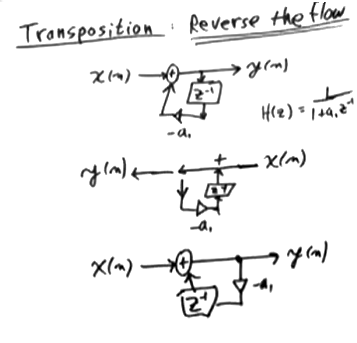
\includegraphics[scale=0.5]{frames/5_a}


\subsection*{DF-1 Biquad}

4:49


$y(n) = b_0x(n) + b_1)x(n - 1)  -
a_1 y(n - 1) - a_2 y(n - 2)
$

*Note process on how he draws it.

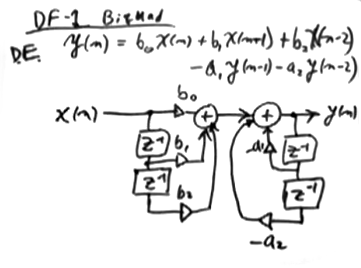
\includegraphics[scale=0.5]{frames/5_b}


\subsection*{DF-2}

around 7:00

Shared delays (more efficient), dangerous intermediate sum that can overflow.

Right: feed forward
left: feed back 
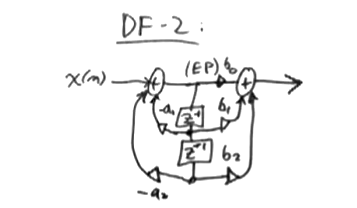
\includegraphics[scale=0.5]{frames/5_c}

\subsection*{Transposed DF-2}
approx 9:00 

\josquote{transposed direct form 2 gets a lot of use}

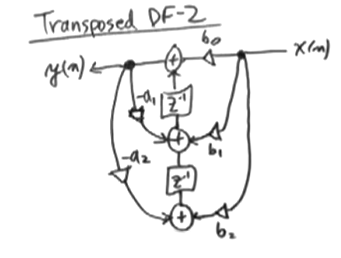
\includegraphics[scale=0.5]{frames/5_d}

\subsection*{FlipLR}
Approx: 11min\\
\josquote{This is the transpose of tapped delay lines... you're summing
into the tapped delay line.}

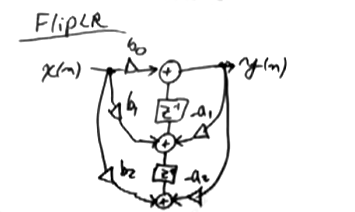
\includegraphics[scale=0.5]{frames/5_e}\\

%\noindent\rule[0.5ex]{\linewidth}{0.5pt}
%\textbf{Class notes: Jan 12, 2016}

Notes for Paul:

- Make a "notes for paul" latex macro

- Learn more about the S-Plane and Z-plane (we will be doing both in this class 
simultaneously)

- Faust filters: many of them are just an impulse sent through a 2nd order filter

- df-1 and df-2 differ by whether or not the zeroes come first or second

\josquote{There is a rate of evaporation of hardware in this vacinity}

\subsection*{Direct Form Filters}

\josquote{Truth is Truth.}

% https://ccrma.stanford.edu/~jos/fp/Direct_Form_I.html

Difference equation: Discrete form of differential equation

- takes a linear combination of the current input, and the past inputs

- can't see the future: causal

- Show up in the numerator of the transfer function

- if it's an FIR, b cf are the impulse response

- vector 'b', sequence of b's, followed by zeros

- TODO: try to see this in terms of convolution (connect it, "last quarters way of thinking about this")

- "running linear combination

- 2 points = two point smoother, running 2 point sum filter

- b-part is only the FIR part, no feedback

- feedback is new this quarter: coudln't do it last semester because the IR is infinite

\textit{(there should definitely be a sidenote thingy for meanderings...
How does one "chart" this lecture?
)} 

- some ways to  model reverbation: ray tracing boundary modelling

\josquote{The gaming industry drives this stuff.}

- impulse response is only accurate for a fixed point fixed source fixed geometry

- reverb is trying to come from everywhere at once

- diffuse field

- image method reverberation: take your room, replicate it. 

- the walls are suddenly made out of mirrors, and you clap: imagine where you'll see those pair of hands. you'll see the hands in 
6 places at first, but you'll realize there are an infinite amount of hands. 

- dual of image method: trakcing a spherical wave that gvoes out when you clap your hands. let it go through
the walls. Find the sound field by adding all the rooms that the soudn wave is in.

-infinite honey comb of image rooms, spherical wave that expands out. take all teh rooms intersecting the sphere 
at that time, and add them together. You'll get a lot of near plane waves, one from every direction. Timing is random
phase is random.

- late in the reverb: diffuse. 

\josquote{You don't localize reverb, you swim in it.} 

- The "diffuse snow field"

\textit{Now were talking about snow clearing infrastructure in Helsinki}

- Impulse response in an ice hotel \\

%\noindent\rule[0.5ex]{\linewidth}{0.5pt}
%Class notes: Jan 14, 2016

\subsection*{Matlab Demo: Time-Domain filters}
* see timedomain.m *

\josquote{Frequency domain is where it's at.}

TODO: learn about Z-transform... what is it?

Julius invented the first filter coroutine in Matlab.
\\
Julius established the b before a design in Matlab.
\\
Filter by default truncates the output signal, so that's why you zero pad.

Confusion about the organization of the book: REALLY simple introduction.

Next tuesday will be the Z transform: Remember that the Z transform is the DFT generalized.

Laplace transform: Generalized case for the fourier transform (continuous time).

BREAK

Talking about Q... shit I wasn't paying attention, but it's an old thing.

-$-3db$ is a factor of $1/\sqrt{2}$

-$Q = \frac{\omega_0}{2 \pi B} = \frac{f_0}{B}$

-$Q \approx$ number of  cycles

-Helmholtz resonance first resonance in guitars %(I think he said that?)

\josquote{I'm 62 years old, and was exposed to unbounded rock and roll when I was a kid}

\section{Analysis of Digial filters}
%\subsection*{Simplest Electrical LPF}

video: vid6.mp4

Practical lowpass electrical filter is an RC filter

\paulhint{First electrical diagram made}

\paulhint{See 6a.png}

Resistor: made out of carbon composite. $V=RI$ Material such that when you 
put a current across it, the current is proportional to the voltage.

\paulhint{This is the second diagram in the page}

\paulhint{See 6b.png}

Capacitors: charged with voltage. Capacitance %spelling?
how much charge can be held in the plates. $Q = cv$

Current is the dirivative of charge.


\paulhint{This is the third diagram in the page}


Inductor: what is this?
\paulhint{This is the fourth diagram in the page}

RLC circuits
\paulhint{See 6c.png for capacitor and inductor}
Approx: 5:36
Analysis of these filters. (Done more formal than necessary).

\paulhint{This is more diagrams. Worth a rewatch maybe?}

Kirchhoff Loop and Node equations: sum of voltages around a loop is zero.

Loops: 

input loope:

$-v_i + v_r + v_c = 0$ \\
$v_i = v_r + v_c$ \\

output loop:
$-v_c + v_0 = 0$ \\

Node: \\
$i_R - i_c + i_0 = 0$\\
$i_c = i_0 + R_c$

Assume output current ($i_0$) is zero.

\paulhint{I'm missing a lot here. Google Kirchhoff}

$V_i = V_r + V_c = V_R + V_0$ \\

$V_0 = V_i - V_R$ \\

Putting it in the laplace domain:\\

$V_0 = V_i - V_R = V_i - IR$ \\
$= V_i - (V_0 c s) * R$

\paulhint{$V_0 c s = I$}

$V_0[I + R c s] = V$

$H(s) = V_0(s) / V_i(s) = 1 / 1 + RCs$

$ = \frac{1/rc}{s + 1/rc} = \frac{1/\tau}{ s + 1/\tau}$

\josquote{Keep swapping in component definitions until you are ready to find the final solution.}


\paulhint{$\tau \stackrel{\Delta}{=} RC$}

$H(s) 
= \frac{1}{1 + R C S} 
\leftrightarrow 
h(t) = \frac{1}{\tau}e^{-t / \tau}$

\josquote{Be comfortable in both the Z plane and the S plane.}

%\noindent\rule[0.5ex]{\linewidth}{0.5pt}
%\subsection*{Generaliszed complex sinusoid}
class notes: jan 19, 2016

$s(t) = e^{-t/\tau}e^{j\omega_0 t}$

%S plane: $s_0 = \sigma_0 + j\omega_0$ and $\simga = -\frac{1}{\tau_0}$

Sample it: $ \leftarrow$

$s(nt) = \alpha * e ^{-nT/\tau_0}e^{j\omega_0 n T}$
$s(nt) = \alpha * (e ^{T/\tau_0})^n(e^{j\omega_0T})^n$


Define: $Z_0 = r_0 e^{j\omega_0}$

i.e, $Ae^{s_0 n T} = AZ_0^n$ s-0dervived and z-derived, respectively.

$Z_0 = e^{S_0 T}$  

\mbox{$s \leftrightarrow z$ map}

$a e^{s_0 t} \rightarrow SAMPLE_t \rightarrow Ae^{s_0 n T}$

$\stackrel{\Delta}{=} A Z_0^m$

$e^T{\sigma_0 + j[\omega_0 + k2\pi fs ]}$\\
$e^T{\sigma_0 T} * e^{j\omega_0}e^{jk}$ \paulhint{not done yet}

This thing aliases, and he jsut wrote a proof why. \paulhint{But... why?}

Add the "strips" together to get the digital domain.



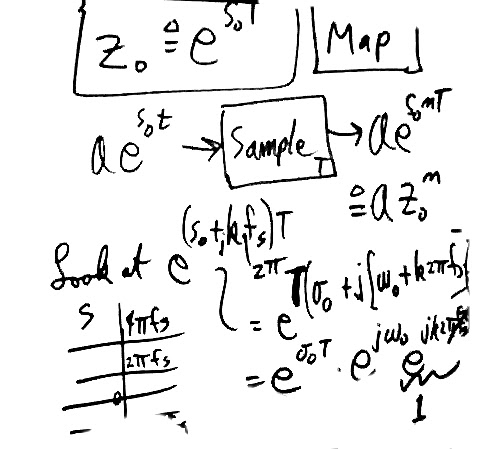
\includegraphics[scale=0.5]{photos/jan17/9a}



$S \leftrightarrow Z$ How?

$z_0 = e^{s_0 T}$ \\

clue: Diff. thm for laplace xf.

\paulhint{how do we prove that a thing doesn't alias?}

$S = \frac{1 - z^{-1}}{T}$

This is called a "Backward Euler", which has the advantage of being causal. The foward Euler (look ahead) needs a + instead of a minus. There's also a Center Euler.

Centered Euler: $\frac{x_{n + 1} - x_{n - 1}}{2T}$

\subsection*{Derivative}

\paulhint{See pictures taken at aroudn 15:35 PST... 9a}


\josquote{For a derivative to exist, it must be unique}

B and F stands for backward and foward.


Four mapping:

sample mapping.

backward euler.

forward euler.

centered approximation. (this onen goes up in order).

\subsection*{Trapezoidal}

step function with samples.  

simple thing is summing the areas x1, x2, x3.

Zero-order integral is to sum the rectangular areas.

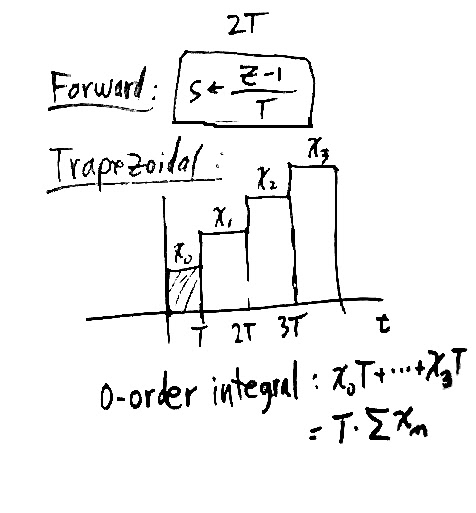
\includegraphics[scale=0.5]{photos/jan17/9b}

First order integral: We want to do a linear interpolation.
Corner to corner. 

We need the areas of the triangles. 

Here is how we do it:

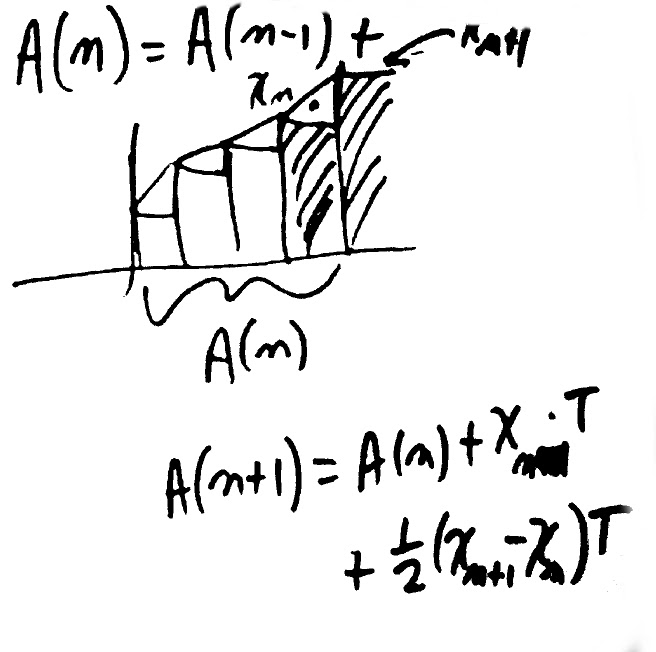
\includegraphics[scale=0.25]{photos/jan17/9i}

This can now be simplified:

$=A(n) + \frac{1}{2}X_{n + 1}T + \frac{1}{2}x_nT$

Trying to see if this turns into the recursion that JOS likes:
$y(n) = y(n -1) + \frac{T}{2}[x_{n + 1} + x_n]$

%Simplifies to form \paulhint{see picture taken at about 3:50. woops didn't catch it.}


Let's take the Z transform using the shift thereom:

$(\frac{1 - Z^ -1}{T})Y(z) = (\frac{1 + z^{-1}}{Z})X(x)$ \\

$H(z) \stackrel{\Delta}{=} \frac{Y(z)}{X(x} = 
\frac{2}{T} \frac{1 - z^{-1}}{1 + z^{-1}}$
Firt order numerical intergration

The first thing you try to do with he S plane (analogue) to the Z plane (digital, discrete) is the bilinear transform. 

Two point average on your signal. 

It's a non-aliasing transformation from the S plane to the Z plane. 


\subsection*{Differentiation}

$x(t) \rightarrow \frac{d}{dt} \rightarrow x(dot)(t) $ \\

$x(t) \leftrightarrow X(s)$
$x(t)(dot) \leftrightarrow sX(s) - x(0) \rightarrow sX(s) $

\paulhint{picture taken at 15:57. Not sure where I am in the lecture 9c }

This is predictive:


$H(z) = \frac{1 - Z^{-1}}{T}$ \\
$H(e^{j \omega T}) = \frac{1 - e^{-j \omega T}}{T}$

\paulhint{see two pictures taken at 16:01 for rest of derivation 9d and 9e}

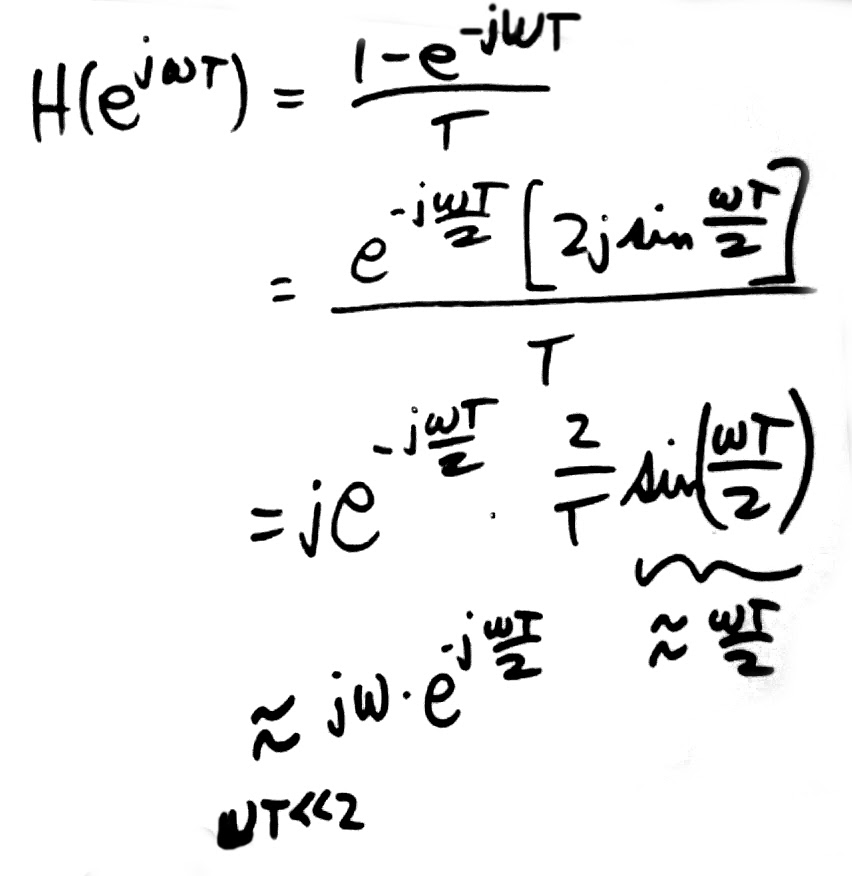
\includegraphics[scale=0.25]{photos/jan17/9d}

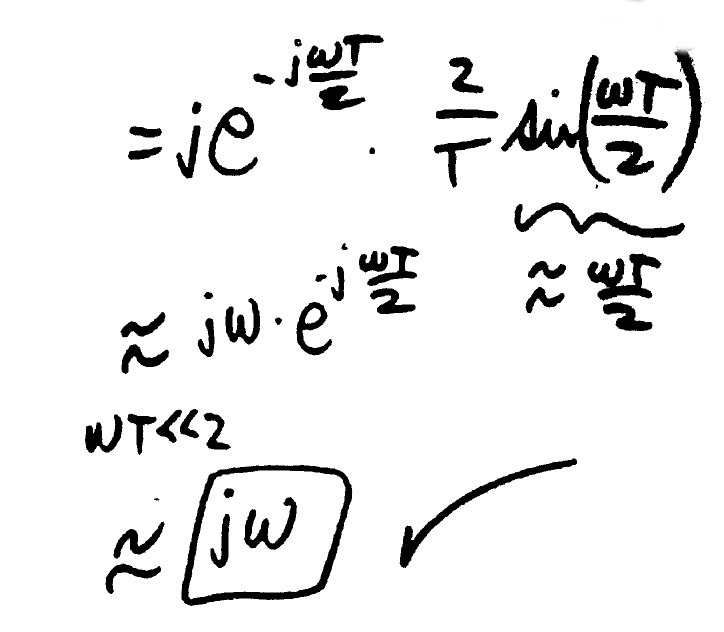
\includegraphics[scale=0.25]{photos/jan17/9e}

\paulhint{look up frequency warping... possibly covered after break}

\josquote{Time was invented to keep everything at once.}

\josquote{Cosmic moments. (Excuse for not doing homework:) It is Written.}

\subsection*{Frequency Warping}

Reminder of what we've seen:

We've seen derivitive of a filter \paulhint{?? this might not be right}

We can approximate the first-order differential equation in many ways. This
is whewre we get the forward/backward euler. 

First order is really nice because it is a noce 1:1 mapping of the S to the Z plane. No aliasing. 

Non-aliasing quarter preserving approximations. 

The really good one is the bilinear transform. 

The ideal differentiator is the + 6db/octave order filter. 

\paulhint{Bilinear transform, backwards euler, etc, are all from the moebius transform, so look up the moebius transform. There's apparently a mindblowing
video on the moebius transform.}

\paulhint{Bilinear transform with anotations (2pt avrage and drvt) see picture taken at 14:32}

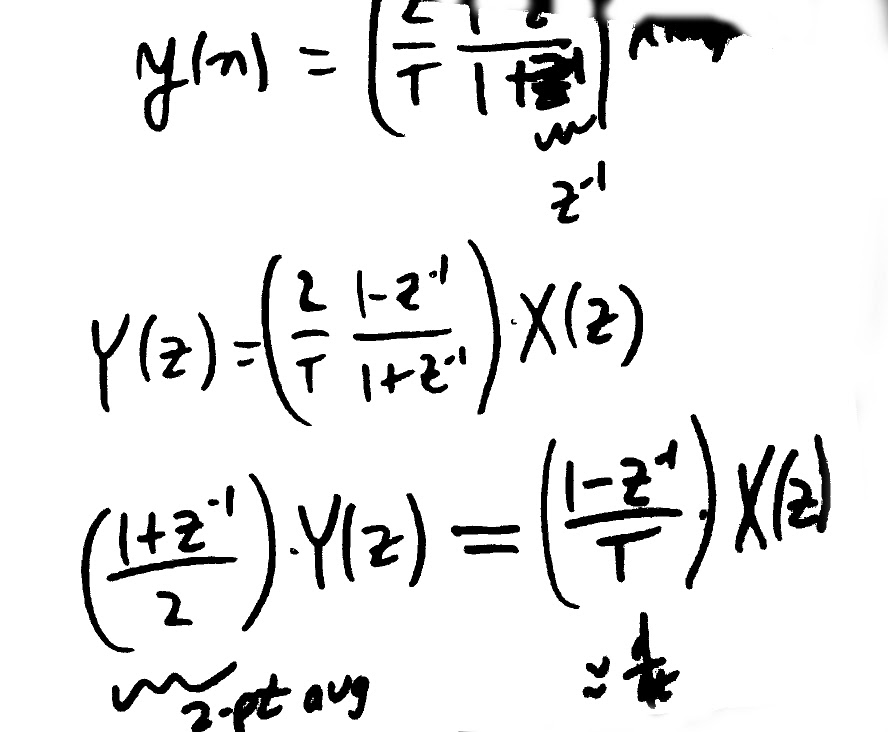
\includegraphics[scale=0.25]{photos/jan17/9j}

\josquote{Bilinear transform is known as the sandwich because it is a BLT (lol)}

\paulhint{Look up trapezoidal rule of derivation.}


graphing s-plane and z plane.

dc is perfectly mapped:

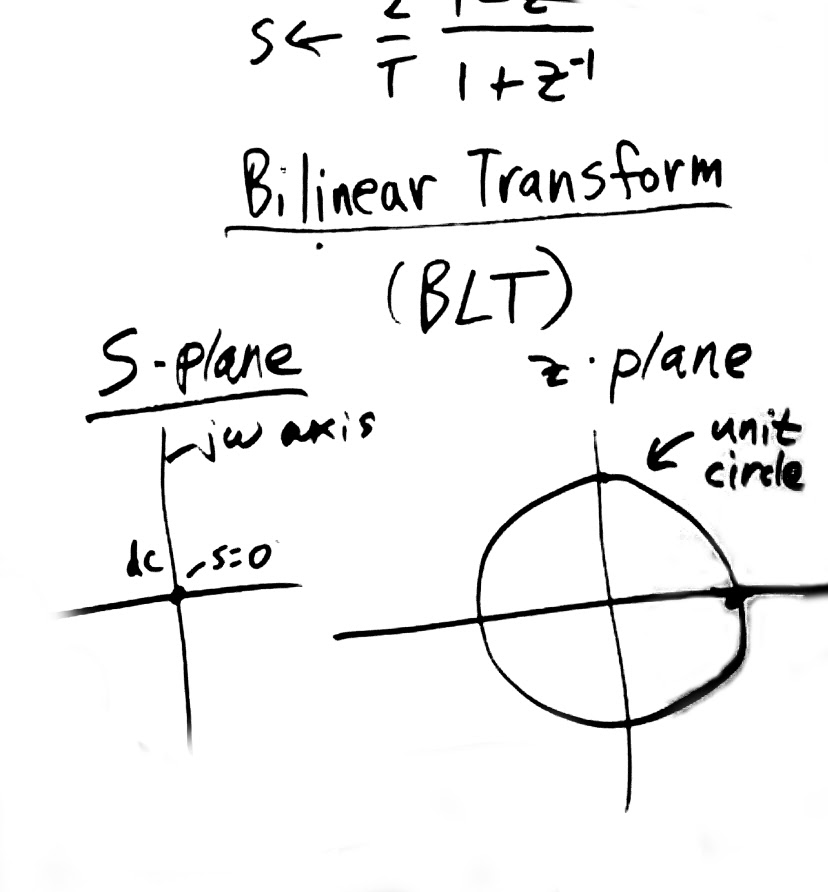
\includegraphics[scale=0.25]{photos/jan17/9f}

half the sampling rate: 

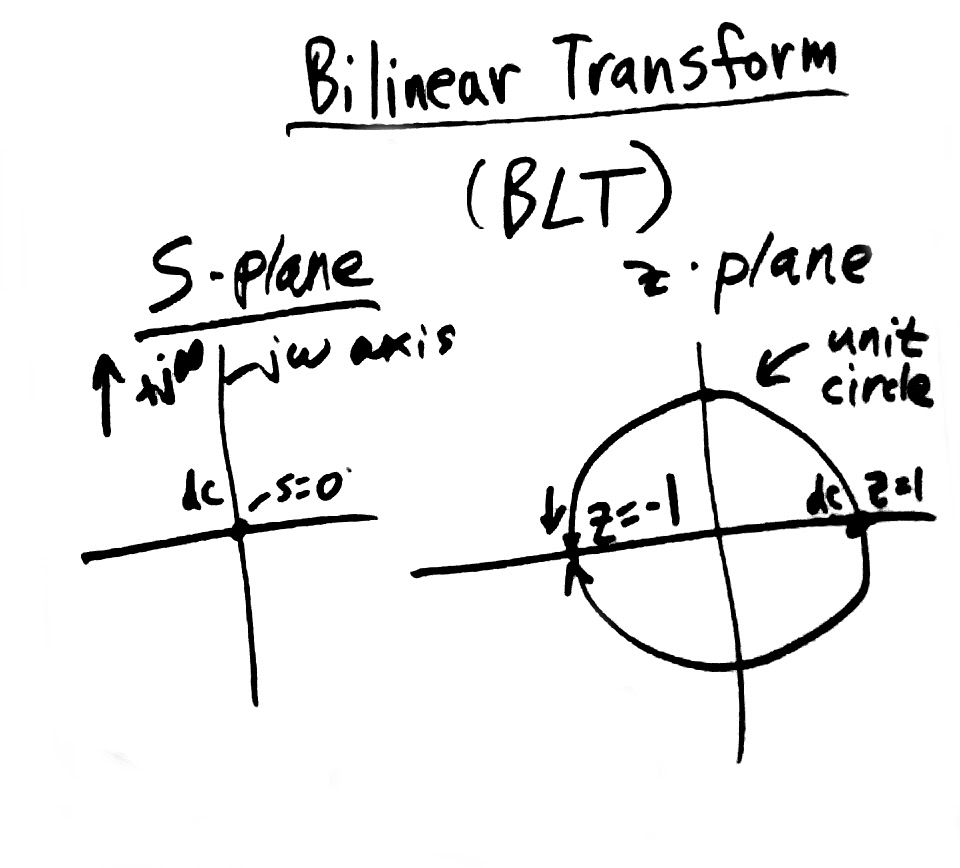
\includegraphics[scale=0.25]{photos/jan17/9g}

BLT: $\frac{s}{a} = \frac{1 - z^{-1}}{1 + z^{-1}}
= \frac{j\omega_a}{a} \stackrel{?}{=}
\frac{1 - e^{-j \omega_a T}}{1 + e^{-j \omega_a T}}$

\josquote{Alpha is just doint frequency scaling, that's all it can do.}
Known true for $w_a = 0, a, \inf$

See picture taken at 16:43 for rest of simplification.

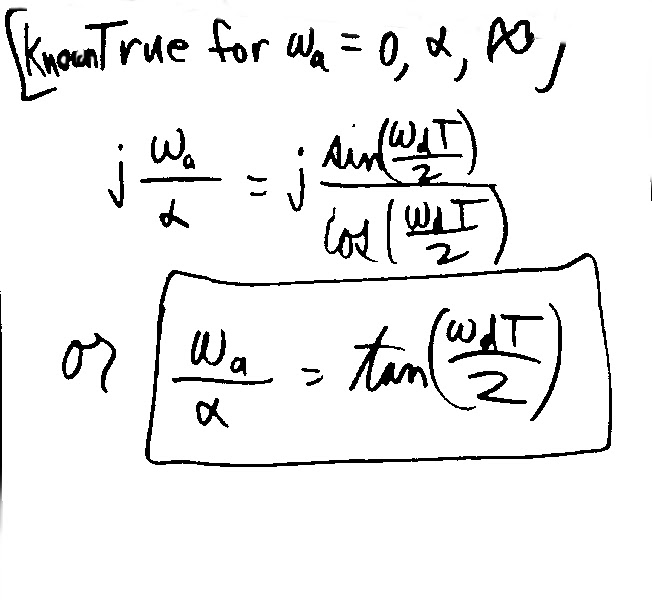
\includegraphics[scale=0.25]{photos/jan17/9h}

\paulhint{This was apparently a homework problem?}


If you change alpha, you change where low frequencies are. 

Alpha is one degree remaining of freedom for tuning a frequency. 

\paulhint{look up the mappings}
\\
%\noindent\rule[0.5ex]{\linewidth}{0.5pt}
%These are notes for vid7.mp4

\subsection*{Low Shelf}

$H(s) = 1 + \frac{B_0}{s + \omega_1}$ \\

where $B_0$ = "boost"   $\omega = 0$

$H(j\omega) = 1 + \frac{B_0 \omega_1}{j \omega_1 + \omega_1}=
1 + \frac{B_0}{1 + j}$

Shelf filters are meant to be used in series.

Hshelf, peaking eq, etc are all multiplicative.


Easily designed, only in the S plane. In the Z plane, things get 
"a bit more gnarly". \\

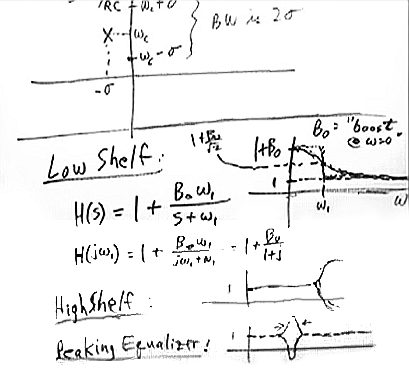
\includegraphics[scale=0.5]{frames/10a}\\
\paulhint{shot 10a taken at 4:16}\\


\subsection*{Bilinear transform}

\josquote{We are creatures of habit. Our brains are constantly trying to automate.}

$S = c \frac{1 - z^{-1}}{1 + z^{-1}}$

Usually, $c = \frac{2}{T}$ where T is the sampling interval.

% TODO: make this an itemize list?
The BLT:
\begin{itemize}
\item{preserves stability.}
\item{preserves order. }
\end{itemize}

\subsubsection*{The mapping (s-plane: left, z-plane: right)}

Critical points to map:
\begin{itemize}
\item{DC is $s = $ when $Z = 1$}
\item{dc maps to dc}
\item{$s = \inf \leftrightarrow z = -1$. infinite analogue frequency maps to
Pi, which means \textbf{No aliasing} at the price of frequency warping}
\end{itemize}

Frequency warping happens at higher frequency. Low frequency axis is in good shape.
It's only the high frequency stuff that gets compressed. As you go up
towards half the sampling rate, equal increments along the unit circle 
correspond to larger and larger increments along the omega axis. 

For some filters this is nice, like LP filters. What used to be a 6db octave is
now a hyper-accelerated rolloff. 

$\frac{1}{S}$ has a zero at infinity. That zero maps to $z = -1$. Your
point at inf maps to half the sampling rate, and you want everything to be
zero there anyways, so it's actually a good thing.

Stop bands are accelerated. If you have a guard band, you do fine. 
Sometimes it's important thatyou don't alias. If you alias a rolloff, 
the aliasing piles up, to the point where it becomes a different function.

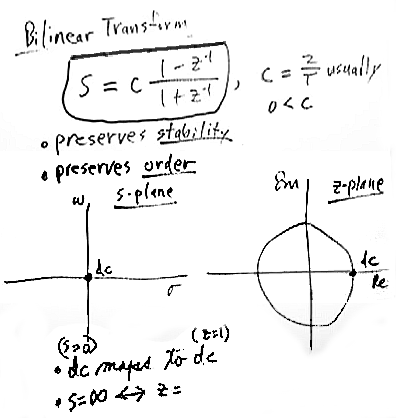
\includegraphics[scale=0.5]{frames/10b}\\
\paulhint{10b is frame taken at 9:05 or so}\\
\paulhint{10c is frame taken at 10:46 or so}


%\noindent\rule[0.5ex]{\linewidth}{0.5pt}
%Class notes for 1-26-16

\subsection*{Null Job Topics}
Null Job: something computers do when there is nothing else to do. 
\begin{itemize}
\item{DFT $\rightarrow$ DTFT $\rightarrow$ FT $\rightarrow$ LT $\rightarrow$ ZT 
$\rightarrow$ DTFT and DFT}
\item{BW of a pole}
\item{Decay Time of a Pole}
\item{Partial Fraction Expansion (PFE)}
\item{Laplace transform}
\end{itemize}

How do you define stability? If the poles are inside the unit circle, it's
stable.
If it's on the unit circle, it is marginally stable. 

\subsection*{Unilateral transform}

\subsection*{Diff Thm transform}

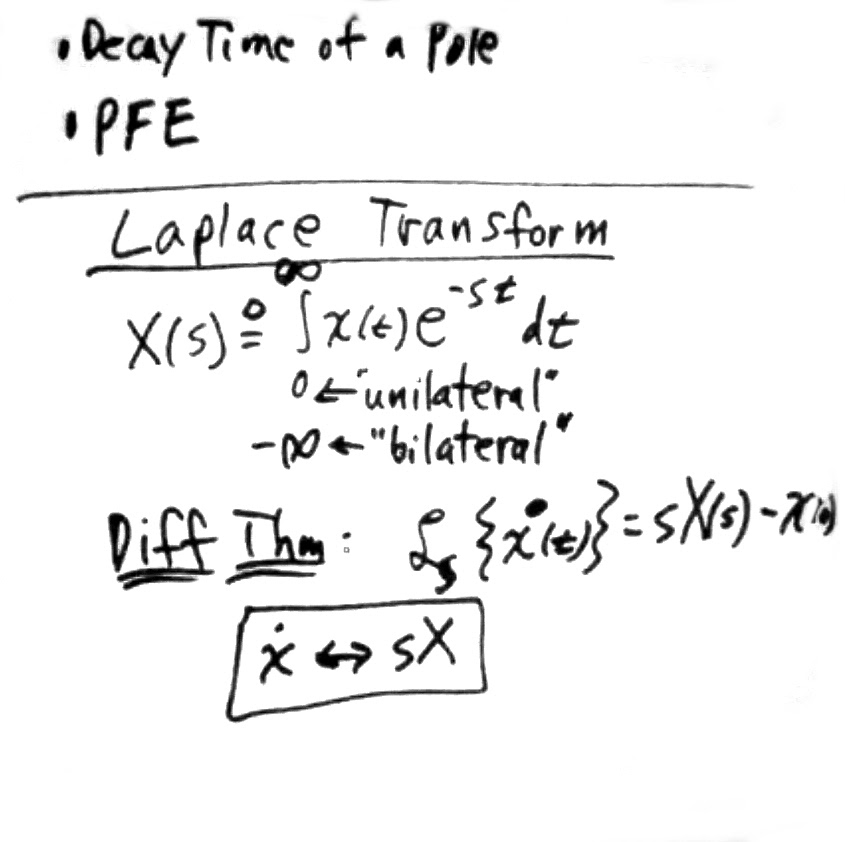
\includegraphics[scale=0.3]{photos/jan26/11a}

This is the counterpart to shift theorem for DFTs. 

\paulhint{Started new recording on a new SD card. woops}

%\paulhint{Little graphic about a "slice", taken at 15:16, 11b}

\subsection*{History of Harmonic Analysis}
History of Harmonic Analysis: darigol (sp?), which goes back to 
Daniel Bernouli. Began summing sinusoidal components "pure vibration". 
A bit later, (name?) began coming up with wave equation for vibrating string. 

You CAN make a progressive wave out of standing waves. 

First thereom: jean baptiste fourier. Had the right idea, but 
didn't have the right proof. He was working on heat diffusion. 

\subsection*{3db Bandwidth of a Pole}
Best to look at the s-plane:

Pole at P. To get the frequency response, plug in $j\omega$ into the transfer
function. 

For s-plane, left is stable and right is unstable. 

\paulhint{TODO: look at s-plane from MDFT book}

What do we need to measure 3db bandwidth? We need magnitude response 
(amplitude response). 
Let's let $P = \sigma_p$

Max is at $\omega = 0$;

%\paulhint{Picture taken at 15:30. he's still drawing though. mark at 1. 11c}

What kind of filter is this? We drew it. 

%\paulhint{Picture taken at 15:33. Note the diagram. 11b}
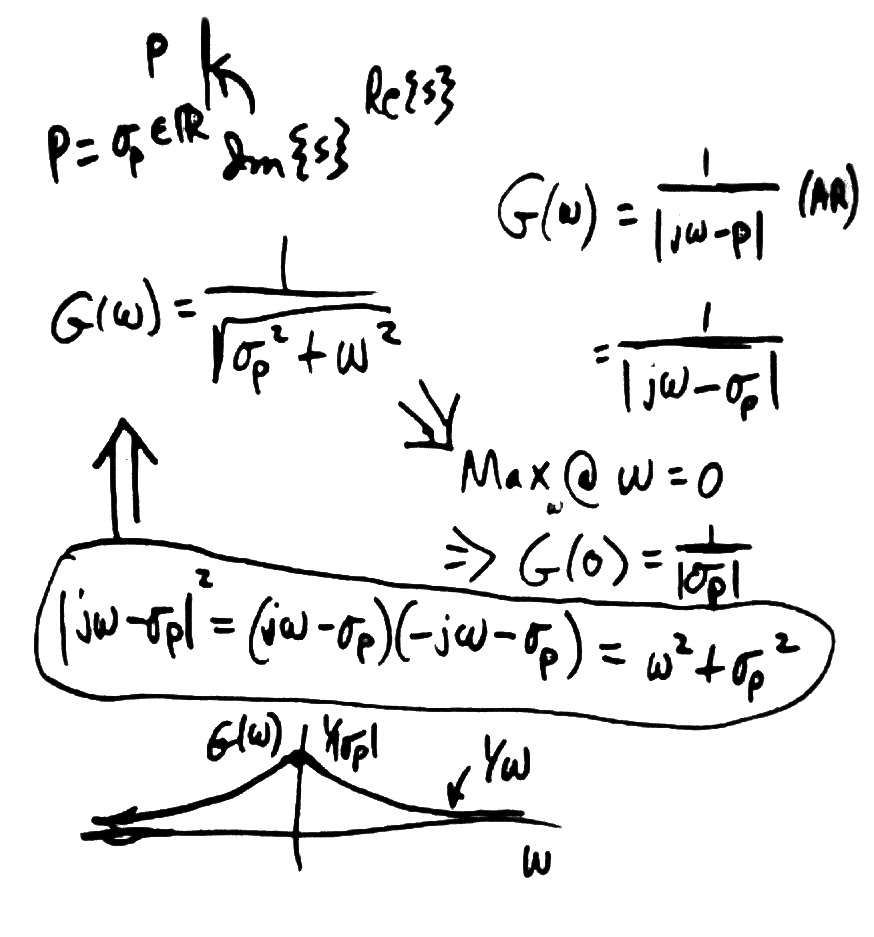
\includegraphics[scale=0.3]{photos/jan26/11b}

Q is center frequency divided by bandwidth. 

$Q = fc/B = 0$

\josquote{When it comes to filters, keep them real. Keep them rational}

\subsection*{Bandpass vs Lowpass}

\subsection*{What does constant Q mean?}

%\paulhint{See picture taken at 15:40. 11c}
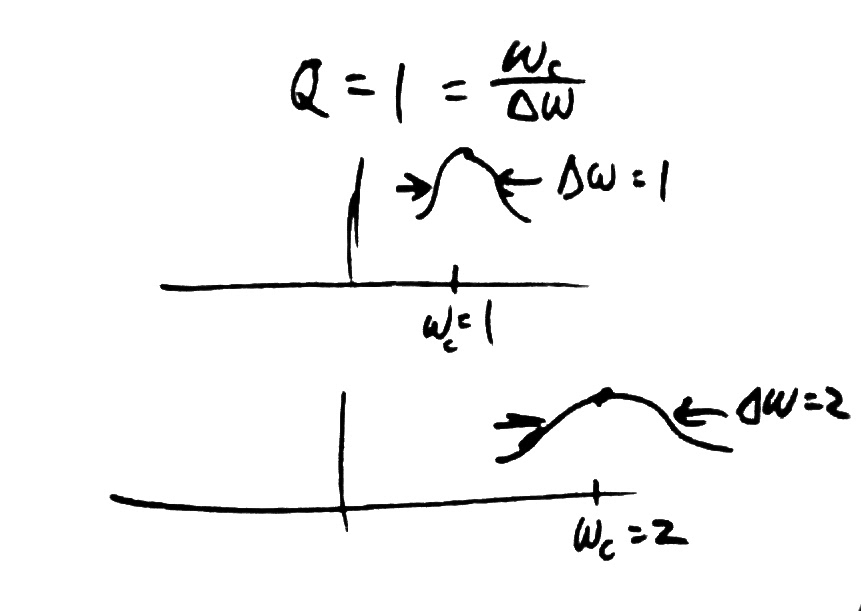
\includegraphics[scale=0.3]{photos/jan26/11c}

\subsection*{Constant Q filter bank}

%\paulhint{See picture taken at 15:41. 11d}
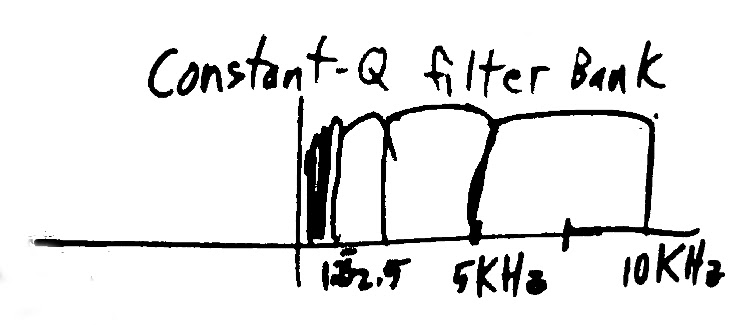
\includegraphics[scale=0.3]{photos/jan26/11d}


\subsection*{Butterworth lowpass}

%\paulhint{See picture taken at 15:43. 11e}
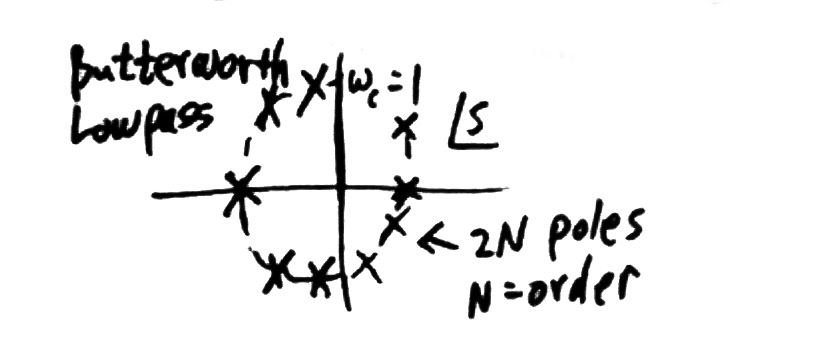
\includegraphics[scale=0.3]{photos/jan26/11e}

\paulhint{What does LHP mean?}

\subsection*{1 Pole Butterworth}

%\paulhint{See picture taken at 15:46. 11f.jpg}
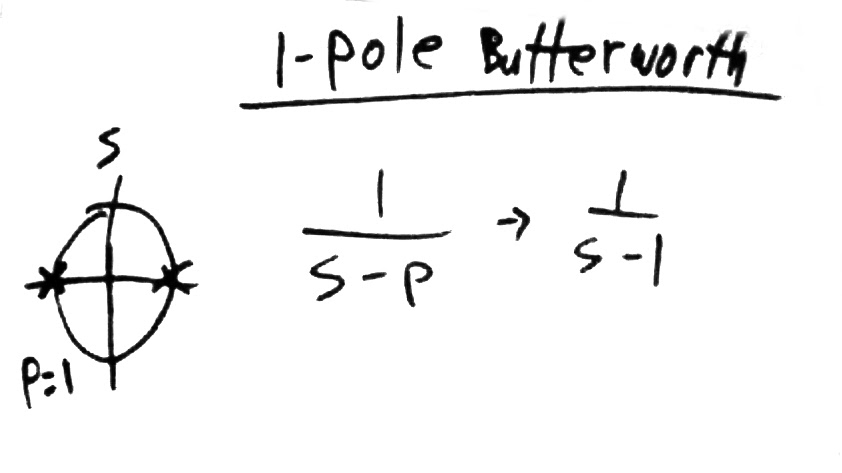
\includegraphics[scale=0.3]{photos/jan26/11f}

This "gives away" the bandwidth of a pole.  
%\subsection*{Frequency scaling}
%
%%\paulhint{See picture taken at 15:48.}
%\paulhint{Another chart taken at 15:49. 11i.jpg}
%
%\subsection*{Finding 3db point}
%
%\paulhint{See pictures at 15:51-2.}
%
%\textbf{Pole bandwidth} = $2 \sigma_p = 2 \pi B$
%
%\subsection*{How to tell if filter is unstable}
%Other ways, without looking at the s-plane and z-plane.
%
%\subsection*{Something}
%\paulhint{See picture at 16:22.}
%
%\subsection*{Something else (laplace transform?)}
%\paulhint{See picture at 16:23.}
%\paulhint{See pictures at 16:25.}
%
%\subsection*{Pole Bandwidth cont.}
%$B =$ bandwidth in Hz\\
%$2 \pi B = 2 \sigma_p$ \\
%
%Let $Z = e^{sT}$
%
%Therefore $Z_p = e^{-pt} = e^{-\sigma_pT} = e^{-\pi B T}$
%
%This is different than the bilinear transform in that it has aliasing. 
%
%$H(s) = \frac{1}{s - p} \leftrightarrow h(t) = e^{pT} =
%e^{-t/\tau}, \sigma_p =-\frac{1}{\tau}$

\subsection*{Complex Resonator}
Move the pole off the DC axis, \\
\paulhint{See pictures at 16:39. 11g}\\
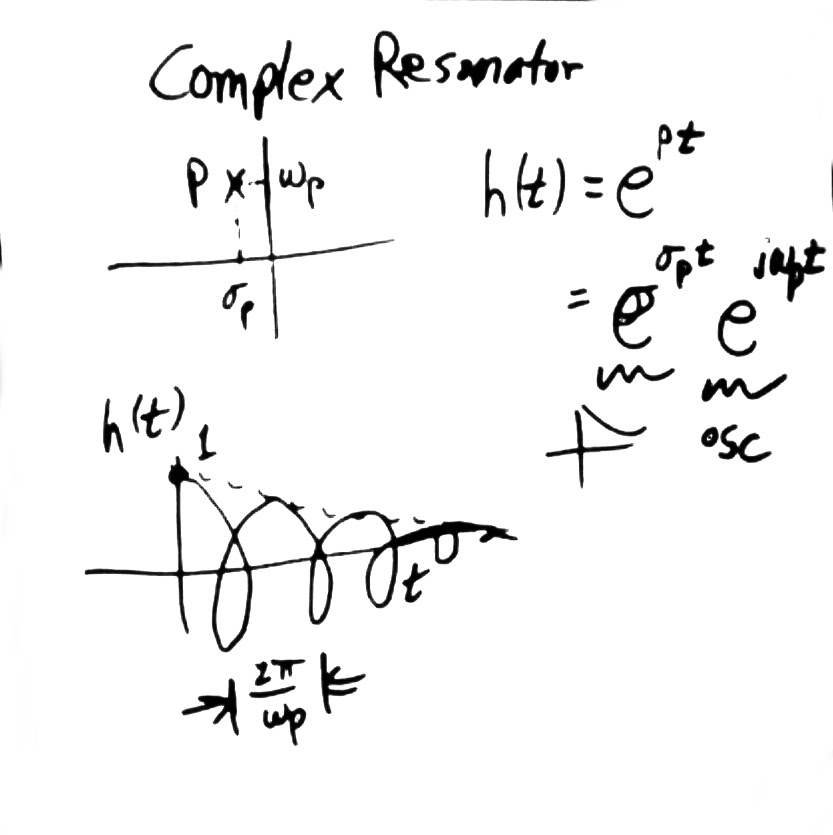
\includegraphics[scale=0.3]{photos/jan26/11g}
%\paulhint{More elaboration at 16:39. 11l}

This is now your basic impulse response resonator. 

Conversion between $t_{60}$ and time constant. It's about a 7th of time constant.
 

%\noindent\rule[0.5ex]{\linewidth}{0.5pt}
%Video notes (vid8.mp4)
\subsection*{Pole-Zero Analysis}

From our difference equation we have:

$Y(Z) = H(Z)X(Z)$

Which can derive the transfer function:

$H(Z) = \frac{B(Z)}{A(Z)}$

\textbf{ex: Our simplest lowpass}:

$y_n= x_n + x_{n - 1}$
$\leftrightarrow Y(Z) = X(Z) + Z^{-1}(Z)$
$H(Z) = 1 + Z^{-1}$


$H(Z) = \frac{B(Z)}{A(Z)}$

General causal LTI filter

\paulhint{frame 12a taken at 3:10}\\
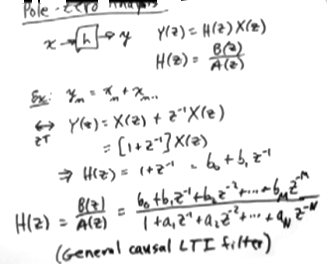
\includegraphics[scale=0.8]{frames/12a}

Without LTI, we don't have a transfer function. 

We pull out $b_0$ to make numerator monic, and write this:

$b_0 \frac{(1 - b_1 Z^{-1})\cdots(1 - b_M Z^{-1})}
{(1 - p_1Z^{-1})\cdots{1 - p_N Z^{-1}}}$


Easier way to write it for pole zero analysis:

\paulhint{frame 12b taken at 5:43}\\
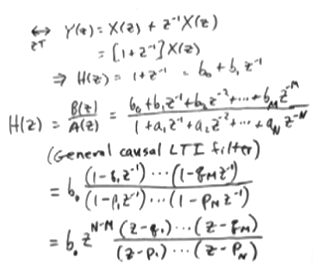
\includegraphics[scale=0.8]{frames/12b}

\subsection*{Freq Response}

The frequency response is the transfer function evaluated on the
unit circle: $H(z)\vert_{z = e^{j\omega T}}$

\paulhint{See eqn at 7:57, 12c}\\
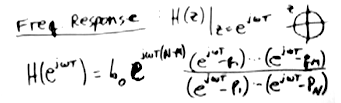
\includegraphics[scale=0.8]{frames/12c}

\subsection*{Graphical Amp Response}

%$G(\omega) = \vert H(e^{j\omegaT) \vert = \vert b_0\vert \cdots $


\paulhint{frame 12d taken at 5:43. use eqn written}\\
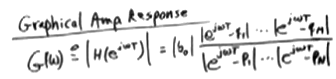
\includegraphics[scale=0.8]{frames/12d}

By graphical, we mean you can now into the complex plane and draw
the unit circle and pick a point on the unit circle. 

To look at our frequency response, we let omega grow from zero to 
half the sampling rate. We can now see what the magnitude frequency response
is as a function of the poles and zeros just looked at as distances. 

$q1$ is numerator

The poles are conjugate pairs (that's what he drew them as). 

The evaluation can done graphically: what is the vector $e^{j\omega T} - q_1$?

It is the arrow from $q_1$ to that point (he draws an arrow). That is the
difference vector. if $q_1$ is added to this difference vector, you get 
$e^{j \omega T}$. 

Normally this method is used for visualizing it graphically in your head. At DC
you are closes to the zero and far from the poles. As you go up, things kind of 
stay the same. when you whip around to the pole, you are going to be 
dividing by a very short distance to that pole, so you can see the resonance that way.
\\
When you fly by a pole, you get a big resonance, or gain peak. 
\\
\paulhint{frame 12e taken at 13:22. mainly for chart}\\
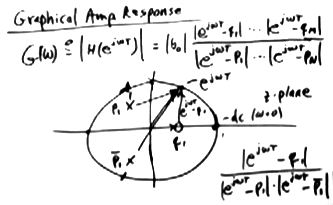
\includegraphics[scale=0.8]{frames/12e}
\\
Traditionally, a zero is denoted with an open zero, and a pole is denoted with an X. 
\\
Typically, we normally go through half the circle because the filter is real
and the negative response is the complex conjugate of the postive frequency 
response.\\

\paulhint{REWATCH: 15:02 is a little unclear (book example). rewatch this and see
if it visually "clicks"} 

\subsection*{Graphical Phase Response}
Same story, but angle instead of magnitude. 

$\theta(\omega) = \angle H(e^{j\omega T})$ \\

We need...\\
Angle $b_0$ will be $0$ or $\pi$ if it is real. \\
Angle for the unit modular constant/term $e^{j\omega T (N - M)}$\\

With amp response, we were multiplying by the zero distances and dividing
by the pole distances, now we want to sum the angles for the zeros, and subtract
for the poles. 


\paulhint{frame 12f taken at 13:22. note the chart.. it is also in the book 
(figure 8.4)}\\
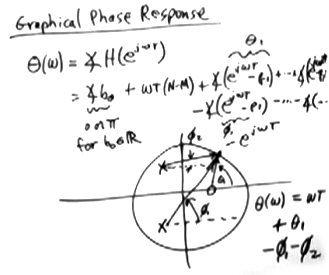
\includegraphics[scale=0.8]{frames/12f}

To reiterate, this approach is really only to visualize what is going on in 
our heads. Computers are more practical.  

In figure 8.5, the phase response has a distorted sinusoidal shape with
the particular point. Qualitatively, our point is the maximum. Why is it the 
maximum? In 8.4, The DC, theta 1 is zero and theta 2 are zero. theta 3, 4 cancel. You
get a zero dc phase. You also get a zero phase at half the sampling rate. 

\paulhint{REWATCH: at around 12:00 he starts explaining how to visually see the
phase, rewatch this as it's a good visualization. You'll want to develop 
this kind of insight.}


%\noindent\rule[0.5ex]{\linewidth}{0.5pt}
%Notes for vid9.mp4

\subsection*{Bode plot of simplest electrical LPF}

The bode plot applies to the amplitude response (magnitude frequency response).

In the s-plane:
$G(\omega) \stackrel{\Delta}{=} \vert H(j \omega)\vert
=\vert \frac{1/\tau}{j\omega + 1/\tau} \vert =
\vert \frac{\sigma}{j \omega + \sigma} \vert 
$

We will plot the magnitude response over a log frequency scale in DB.

When $\omega = 0$, the gain is 1.

0 db for low frequencies, until $\omega$ becomes comparable to $\frac{1}{\tau}$

When we reach $\sigma$, what is our gain? $1/\sqrt{2}$, which is -3db. 

For $\omega > \sigma$, it is 6db/octave rolloff. Our bode plot looks like a 
half decent lowpass filter! It's got a nice pass band, and a well dfined -3db 
point. This is cascadable, so they can be stacked to get a steeper rolloff.

\paulhint{frame 13a taken at 3:26}

\subsection*{Pole zero diagram}
Recall the pole-zero plot:

What is the bandwidth of that pole? 

Bandwidth is interval between -3db points. We just derived that $\sigma = -3d$,
so we can just rotate to the $j\omega$ axis, which is why the s-plane
more enjoyable than the z-plane. 

You can say that in the z-plane your 
frequency axis is the unit circle, and if you straighten it out you'll
get the s-plane. The $j\omega$ axis is a great circle in the extended
complex plane; if you put everything on a sphere, then the $j\omega$ axis
is a circle. 

\section{Digital Filter Design}
%Notes for vid10.mp4

\subsection*{Analog filters}

2 big ways to talk about analog filters: convert analog filter to
digital filter, or estimate their coefficients. 

The anlogue filter is typically easier to talk about because it lives
in the s-plane for it's transfer function:

\begin{align*}
    H(s) = \frac{B(s)}{A(s)} = 
    \frac{
        b_0 s^N + b_1 s^{N-1} \cdots + b_M
    } {
        s^N + a_1 s^{N-1} \cdots a_N s + a_N
    }
\end{align*}

\subsection*{Freq Resp}

Evaluated on the $j\omega$ axis

\begin{align*}
    H(s) \vert_s=j\omega = H(j\omega)
\end{align*}

\subsection*{Power Response}

\begin{align*}
    P(\omega) 
    &\stackrel{\Delta}{=} G^2(\omega) 
    \stackrel{\Delta}{=}
    \vert H(j \omega) \vert^2 \\
    &= H(s)H(-s)\vert_{s=j\omega} \\
    &= H(j \omega)H(-j\omega) 
    &= \overline{H(j \omega)H(-j\omega)} (real filter)
\end{align*}

For a real filter, we can fit a rational polynomial to the power response, 
and do what is called a \textit{Spectral Factorization} to find the
stable poles, and the unstable poles will be on the other side.\\

\textbf{Example LPF}\\

\paulhint{see frame 14a taken at 8:02 }\\
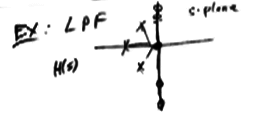
\includegraphics[scale=0.5]{frames/14a}\\
Poles will be in the left hand plane (stable). 

Zeros anywhere it wants. 
Most of the time zeros are at infinity, but more aggressive filters will have
finite zeros.

This is a lowpass filter: graphical method of the impulse response:

Start at DC, take the product of the lengths of all the zeros and take the
products of all the lengths of the poles. As you get away from the poles,
you'll be dividing by large distances to the poles.

Until you leave the "zone" of poles, it's hard to see really where the minimum 
is. 

These are the poles and zeros of $H(-s)$. 

$H(-s)$:
\paulhint{see frame 14b taken at 8:51 }\\
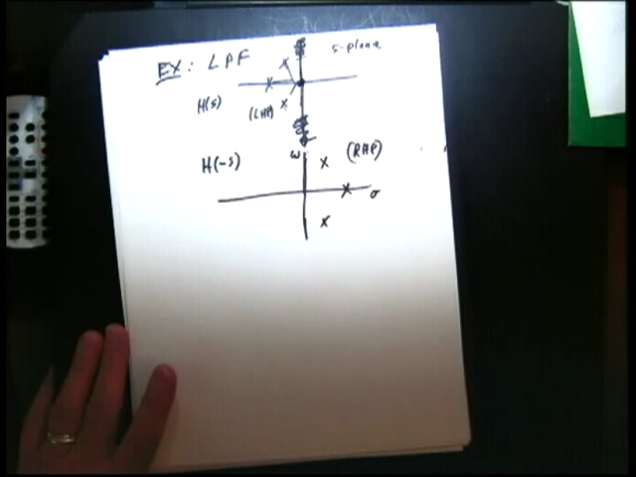
\includegraphics[scale=0.5]{frames/14b}\\

Poles exist in right half plane (RHP). Negative poles in previous graph
exist in left half plane (LHP). 

$H(-s)$: what it relfects about both sigma and the $j\omega$ axis: it's a
double flip, but there's an updown symmetry because the filter is real. Because
it's real, it has complex conjugate symmetry, so the updown flip doesn't do an thing.

\paulhint{TODO: read up on symmetry}

For real filters, you can think of them as being flipped left/right.

When you multiply, you get a symetric constellation of poles:
$H(s)H(-s)$

That is what the power response looks like for a lowpass filter. A generalized
power response. We've taken the power response and extended it to the entire 
complex plane by means of analytic continuation. 

\paulhint{See 14c at 10:22}\\
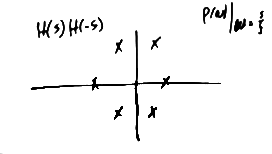
\includegraphics[scale=0.5]{frames/14c}\\

Since P is even in $\omega$, that implies that it is of the form:

\paulhint{See eqn 14d 12:03. TODO: maybe TeX this out?}\\
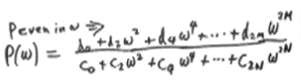
\includegraphics[scale=0.5]{frames/14d}\\

It is not going to have any odd powers of omega. 

We aren't assuming it is monic for generality. 

If there was a cubed term, there would be an asymmetry about zero on the
$j\omega$ axis, and it could not be a real filter. TO be a real filter,
it has to have a symmetric magnitiude, and you square it to get the power
response. \\

This is another example why the S-plane is easier to work in: we don't
get this on the unit circle, and we don't get this nice disapperance of
odd order terms. 

\subsection*{LPF Design}

Passband: Desired response (gain) is $P(\omega) = 1$. \\

Error: 
\begin{align*}
    E(\omega) &\stackrel{\Delta}{=} P(\omega) - 1\\
    &= \frac{D(\omega)}{C(\omega)} - 1 \\
    &= \frac{D(\omega) - C(\omega)}{C(\omega)} \\
    E(\omega)C(\omega) &= D(\omega) - C(\omega)
\end{align*}

Lets start using up degrees of freedom to get what we want. 

We can't set $E$ to zero, because there is no stop band. 

To avoid degenerecy (ie make it a lowpass) will require N > M. This means
D cannot be equal to C. \\

In audio, signals are concetrated around DC, the sampling rates are very large,
and we hear on a more or less log freq scale, and so the first octaves are
the most important. You really want to concentrate on a good filter at the low
frequencies. \\

Let $E(0) = 0 \rightarrow D(0) = C(0) \leftrightarrow d_0 = c_0$ \\

By insisting on exact unity DC gain, it's very often important that your
DC gain be exactly 1; anything greater than 1 is a growth of DC, anything less
is a loss of DC. In physical modelling, this is very important.\\

The next thing want to do is to set the slope to zero at DC: $E'(0) = 0$.

Let's differentiate it:

\paulhint{See the eqn at 14e} 
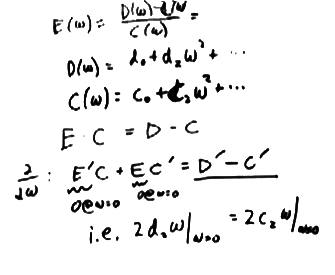
\includegraphics[scale=0.5]{frames/14e}\\

This is already true because it's even. Take the second derivitive $E''C$.

\paulhint{See the eqn at 14f 24:55} \\
\paulhint{Continuation of 14f... 14g 28:35}\\
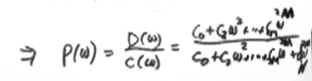
\includegraphics[scale=0.5]{frames/14f}\\
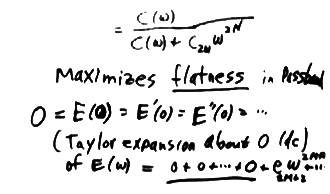
\includegraphics[scale=0.5]{frames/14g}\\

One leftover term forces it to be a lowpass. This maximizes flatness in
the pass band from DC. Flatness: how many terms in the taylor expansion you set to zero:
\begin{align*}
    0 = E(0) = E'(0) = E''(0) = \cdots 
\end{align*}

\paulhint{LOOK UP: Pade approximation}


%\noindent\rule[0.5ex]{\linewidth}{0.5pt}
%Notes for video 11.mp4
\subsection*{Butterworth Filter}

Choose $C(\omega)$ for maximum flatness at $\infty$.

We want the taylor expansion about infinity to be maximum flat. 

Work with $P(1/\omega)$ and go for maximum flatness at "new DC". \\
You want a maximally flat approximation to zero. 
\begin{align*}
C(\omega) &= 1 \\
C(\omega) &= \frac{1}{1 + C_{2N}\omega^{2N}}
\end{align*}

\paulhint{See frame 15a taken at 3:24}\\
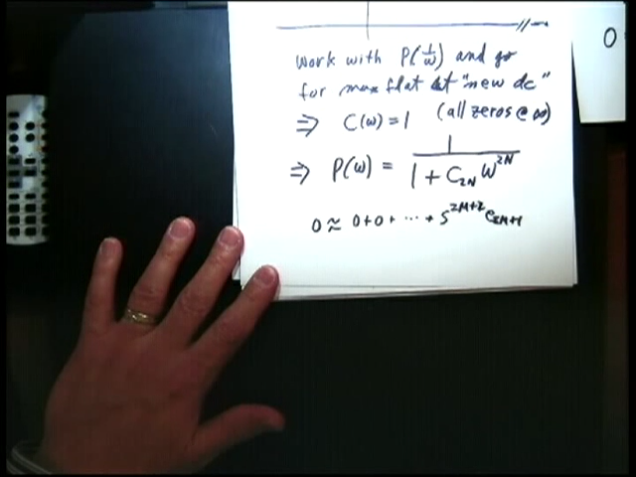
\includegraphics[scale=0.5]{frames/15a}


It's already a taylor series approximation starting at $2M + 2$.

Cutoff frequency gets changed by changing the C coefficient. \\

The more zeroes you have at inifity, the steeper the rolloff.  \\

\subsection*{Good for phase response}


\paulhint{See frame 15b taken at top chart.}\\
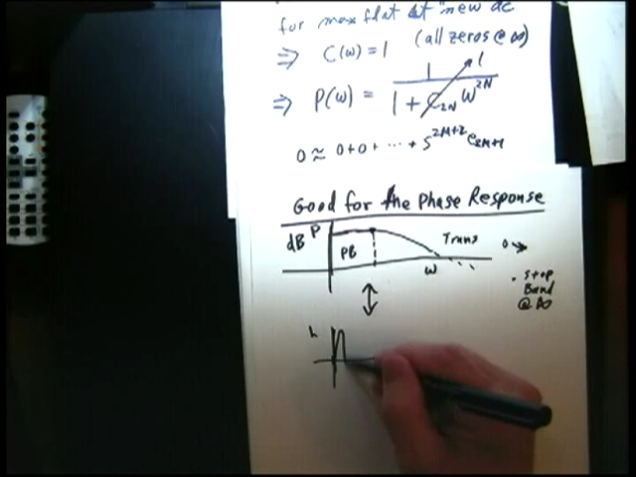
\includegraphics[scale=0.5]{frames/15b}

\begin{itemize}
\item{Maximally flat pass band, and a maximally slow transition band. }
\item{There isn't really a stop band, it's all transition band.}
\item{Stop band is at $\infty$, the only place you make it to zero. 
    Maximally gentle lowpass filter.} 

The impulse response is going to be short:

\paulhint{See frame 15c. Short imp} \\
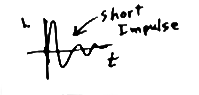
\includegraphics[scale=0.5]{frames/15c}

\item{Short means, there isn't much phase distortion.}

\item{Suppose you put an impulse into the LPF filter: 

\paulhint{See frame 15d. Little diagram with LPF box} \\
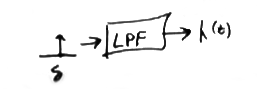
\includegraphics[scale=0.5]{frames/15d}
}

\item{Intuitively, the filter will take the broadband click and output a narrow
    band click. It should not ring. If you hear a ring, it is phase distortion. }

\item{The ideal lowpass filter has a "corner", and the sync function rings like
crazy at the cutoff. Think of that as delaying those components. 
Group delay has a huge spike at cutoff frequency and polezero diagram.}

%\paulhint{See frame 15e. Little diagram with sync box, pole zero 
%diagrams, and group delay} \\
%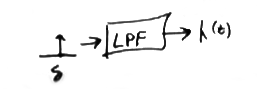
\includegraphics[scale=0.5]{frames/15d}

\item{In the class of filters you often use, butterworth is the most friendly and
    gentle to use. It's a nice smooth warm thing. Good thing to try first.}

\item{
$P(\omega) = \frac{1}{1 + \omega^{2N}}$ \\
$H(s)H(-s) = P(\omega) = P(\omega) \vert_{\omega = \frac{s}{j}}
= \frac{1}{1 + (\frac{s}{j})^{2N}}
$ \\
}

\item{You might recognize this as roots of unity. A bunch of poles at the roots
of unity. Unit circle in the S-plane, which is where the poles of the butterworth
filter lie.
\paulhint{See frame 15e. chart} \\
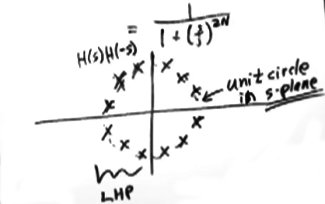
\includegraphics[scale=0.5]{frames/15e}
}

\item{Poles are at 2nth roots of unity for odd N, else rot($pi/wN$).}

\item{ Take the spectral factorization:  \\
LHP: \\
$H(s) = \frac{1}{(s - p_1) \cdots (s- p_n)}$
\paulhint{See frame 15g. for H(s) eqn} \\
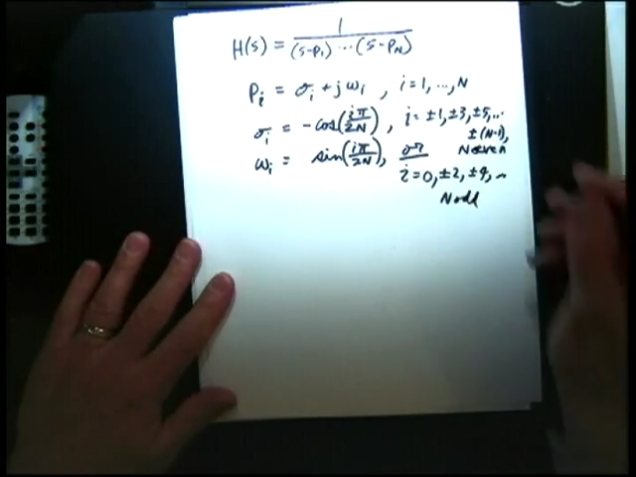
\includegraphics[scale=0.5]{frames/15g}
}

\item{Intuitively, $N =1$, real pole, and minus s is mirrored at roots of unity.}

%\paulhint{graph is being written for N = 1 15h}\\
\item{
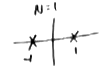
\includegraphics[scale=0.9]{frames/15h}
}
\item{
When $N = 2$, you get into trouble when you get roots of unity would be like
the DFT case, so you rotate the poles:
}
  
\item{\paulhint{graph is being written for N = 2 15i}\\
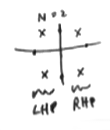
\includegraphics[scale=0.9]{frames/15i}
}

\end{itemize}

\subsection*{Series Biquad Realization}

The poles are in closed form, so we can easily take a series biquad realization.

\paulhint{Stonehenge like graphics. screenshot taken at 23:38 15j}

Elliptic function filter design are hard. Will NOT be covered in class. 


\paulhint{graph is being written for N = 2 15j}\\
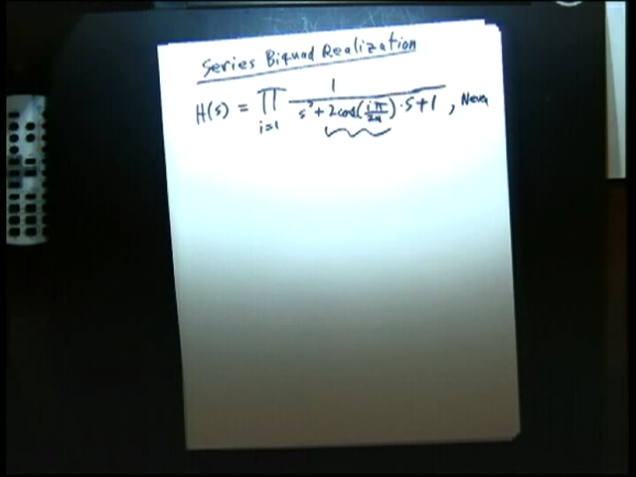
\includegraphics[scale=0.9]{frames/15j}\\

%\noindent\rule[0.5ex]{\linewidth}{0.5pt}
%\subsection*{Something or other}
Class notes: tuesday, Feb 2.

Misc. class points that I was able to take down

\begin{itemize}

\item{Ringing: if you "pulse" it, does it ring? This means that you'll hear a sinusoidal frequency.}
\paulhint{TODO: look up butterworth wiki page. we are looking at it right now}

\item{The number of poles is always equal to the number of zeros at infinity. }

\item{Repeated poles and repeated zeros are difficult to deal with numerically. It is "numerically ill-conditioned"}

\item{There's a good chart of various orders of butterworth filters on the wiki with maximally flat. 
These are Bode plots.}

\item{Bode plots are very audio-friendly. "log-log".}

\item{When the "Pole breaks"? Along the j omega axis, you pass the imaginary coordinate part of the pole.}

\end{itemize}

\subsection*{Bode Plots}
Our transfer function:

\begin{align*}
H(s) = \frac{1}{s - \sigma_p}
\end{align*}

Sigma is the real part, omega is the imaginary part. 

Set sigma to zero to get j omega axis:

\begin{align*}
H(j \omega ) = \frac{1}{j \omega - \sigma_p}
\end{align*}

% \begin{align*}
% G(\omega) = H(j \omega ) = \frac{1}{j \omega - \sigma_p}
% \end{align*}


\paulhint{See picture taken at 15:28}\\

We do a graphical derivation:\\
\paulhint{See picture taken at 15:30}\\


More generally\\
\paulhint{See picture taken at 15:33}\\

\paulhint{See better picture taken at 15:36}\\

\paulhint{I'm still not getting the visual perception of poles/zeros. TODO: look this up}\\

\paulhint{TODO: look up Q and memorize the eqn. Remember that you know this from a 
musical/applications perspective.}\\

\begin{itemize}
\item{Butterworth filter is notoriously non-ringing.}
\item{A one pole filter cannot ring.}
\end{itemize}

Elliptic vs Butterworth

\paulhint{See picture taken at 16:17. Try to figure out what it means as you don't know it yet}



%\noindent\rule[0.5ex]{\linewidth}{0.5pt}
%Video notes: vid12.mp4

\subsection*{Example}
Second order example.  N = 2

We expect that poles aroudn the unit circle at $H(s)H(-s)$.

This is the N-even case, so the poles are rotated so you don't get 
poles on the $j\omega$ axis:

We expect the angle to be 3pi/4 (see chart)

\paulhint{see frame 17a taken at}\\
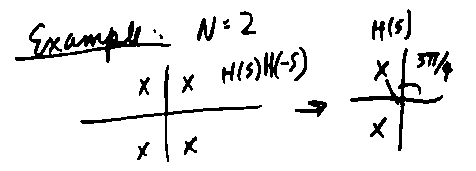
\includegraphics[scale=0.5]{frames/17a}\\

We can express $H(s)$ as a cascade of these poles:


\paulhint{see eqn 17b taken at 1:42}\\
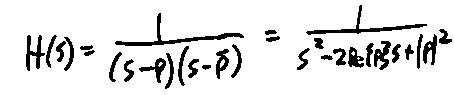
\includegraphics[scale=0.5]{frames/17b}\\

What is P? We can write it as $e^{j3/4pi}$ which means the real part is
$cos(3\pi/4)$, which is equal to $-1/\sqrt{2}$. 

\paulhint{see eqn + graph 17c taken at 3:38}\\
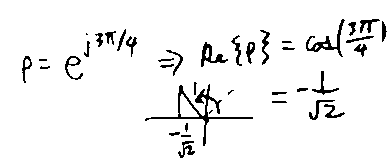
\includegraphics[scale=0.5]{frames/17c}\\

Now that we have foudn that middle coefficient, we can rewrite 
the transfer function as:

\paulhint{see eqn + graph 17d taken at 4:09}\\
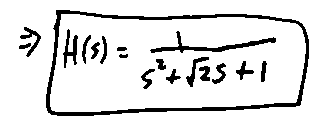
\includegraphics[scale=0.5]{frames/17d}\\

\subsection*{Go Digital}

When you map the splane to the unit circle, the rigthand plane maps
to the exterior unit circle, and the lefthand plane maps to the interior unit circle,
which is only true for $c > 0$, otherwise they change places if it is negative.

\paulhint{LHP and RHP 17e taken at }\\
\includegraphics[scale=0.5]{frames/17d}\\

We plug in the bilinear transform to:

\paulhint{17f taken at 6:16}\\
\includegraphics[scale=0.5]{frames/17f}\\

"Unit term" is just one. 

Now we want to get it into a better form. 

First we multiply the numerator by $(1 + z^{-1})^2$:

\paulhint{17g taken at 7:16}\\
\includegraphics[scale=0.5]{frames/17g}\\

Multiply this out to collect powers of z inverse:

\paulhint{17h taken at }\\
\includegraphics[scale=0.5]{frames/17h}\\

Collect these things together. Find all the constant terms. 

\paulhint{17i taken at 7:16}\\
\includegraphics[scale=0.5]{frames/17i}\\

We're still not quite done, becuase we need a monic denominator. So we pull
the first term out to make it a gain:

\paulhint{17j taken at 10:12}\\
\includegraphics[scale=0.5]{frames/17j}\\

We've done a second order butterworth filter, and we have digitized it.

Now, let's set the cutoff frequency $\omega_c$

\subsection*{Set the cutoff frequency to $pi/2$}

To do that, we have to normalize it. TO do that, you need to look
at the biliear transform mapping:

\paulhint{17k taken at 11:53}\\
\includegraphics[scale=0.5]{frames/17k}\\

We're normalized, so $\omega_a = 1$. We want $\omega_d T = \pi/2$

This implies $e^{-j\omega_d T} = e^{-j\pi/2} = -j$.

We start with this equation:

\begin{align*}
j\omega_a = c \frac{1 - e^{_j\omega_d T}}{1 + e^{-j \omega_d T}}
\end{align*}

And we factor out just like we did with the simplest lowpass filter:

\paulhint{17l taken at 13:39}\\
\includegraphics[scale=0.5]{frames/17l}\\

Our final equation is

\begin{align*}
j\omega_a = c j \tan(\omega_d T / 2)
\end{align*}

This is a nice simple expression to work with, as the j's cancel. 

The analogue frequency axis relates to the digial frequency axis in this way:

\begin{align*}
\omega_a = c \tan(\omega_d T / 2)
\end{align*}

We desire $\omega_a = 1$  to map to $\omega_dT = \pi / 2$, so this all equals
$c \tan(\pi/4) = 1$

Therefore, our halfband lowpass filter (cuts off at half the sampling rate) is:

\begin{align*}
H(z) = \frac{1}{2 + \sqrt{2}} \frac{(1+ z^{-1})^2} {1 + 
(\frac{2 - \sqrt{2}}{2 + \sqrt{2}})z^{-2}
}
\end{align*}

We half two zeros at hafl the sampling rate, and imaginary poles on the imaginary
axis in the z-plane. This is a butterworth filter that has a -3db at 
$\omega_d  = \pi/2$. 

\paulhint{17m taken at 16:22}\\
\includegraphics[scale=0.5]{frames/17m}\\

\subsection*{Check our Work}

dc gain = $H_d(1) = \frac{1}{2 + \sqrt{2}} 
\frac{2^2}{1 +
\frac{2 - \sqrt{2}}{2 + \sqrt{2}}
} =
\frac{4}{2 +\sqrt{2} + 2 - \sqrt{2} } = 1
$

DC is one as expected.

Half the sampling rate is easy to check, you plug in -1 and you get two zeros.

You can check that the cutoff freq is exactly -3db:

\paulhint{17n taken at 18:21}\\
\includegraphics[scale=0.5]{frames/17n}\\

(he skipped a couple of steps here)

%\noindent\rule[0.5ex]{\linewidth}{0.5pt}
%Class notes 2-4-16

%\noindent\rule[0.5ex]{\linewidth}{0.5pt}
%\begin{itemize}
\item{Class notes: Tue, Feb 9}
\item{\subsection*{Spectral Centroid}}

Basic idea: spectrum (magnitude or magnitude squared), and you're looking for
the balance point of the spectrum.

\paulhint{chart at 15:06}


With the equation:

\paulhint{eqn at 15:06}

\subsection*{Power Spectral Centroid}
\paulhint{eqn at 15:06}

this eqn has normalization


with L2 norm:

\paulhint{eqn at 15:08}

\item{This allows us to use differentian.}

\item{Normalization in frequency domain is normaliztion in time domain (paricbles thereom?)}

\paulhint{eqn at 15:09}

\item{What is the application for this? Great automatic definition of brightness in a track.}

\item{How to recover the spectral envelope? You use the cepstrum. }

\item{CEPStrum and SPECtrum are related (flip words).}


\item{Pitch adaptive MFCCs are rare/nonexistant. usually a fixed pitch}
\item{16kHz (sometimes 12kHz): standard speech recgonition SR. 8khz: phone SR}
\item{With MFCCs you get the whole envelope, and all the formants, up to 6 resonances with 16kHz}
\item{8kHz: 3, 4 resonances for speech}
\item{We only need as many resonances for intelligibility, in reality they go to infinity}
\item{How do you do this in the time domain?}
\item{What's the differences between windowed cepstrum vs spectral peaks with interpolation?
These are two methods. Cepstrum gets some pyschoacoustic weighting.}
\item{Another contender: LPC - linear predictive coding: a particular kind of spectral envelope that fits an
all pole filter to the spectrum. It is a peak-biased spectral envelope. Even more pyschoacoustic thrust.}
\item{LPC is an all-pole model. (what is an all-pole filter?)}
\item{All these will be covered in 421!}
\end{itemize}

%\noindent\rule[0.5ex]{\linewidth}{0.5pt}
%\begin{itemize}
\item{Class notes: 2-11-16}
\subsection*{Matlab demo}

\item{
zp2tf: zero pole to transfer function, gives us our A and B coefficients.
}

\item{
Frequency vector returned by freqs is useful for plots. 
}

\item{
Phase plot: how to convert phase to time delay? Find the slope of the phase (phase delay):
\begin{align*}
-\frac{\theta(\omega)}{\omega}
\end{align*} 
}

\item{
Plotting group delay: plot(w(1:end-1), -diff(unwrap(angle(H)))/w)
}

\item{
We have 1400 samples of delay at the corner frequency
}

\item{
There should be a filter designed to be similar to the butterworth filter, so you can
call it "I can't believe it's not butter".
}

\item{
Convert to radians: freq * 2 * pi
}

\subsection*{Julius}
\item{
FDA tool: Filter Desgin and Analysis
}

\item{
Tool only available in MATLAB, not Octave
}

\item{
Able to generate Matlab code.
}

\item{
Maximally flat: for group delay it's called a Bessel Filter. For butterworth it's something else... (phase?)
}

\subsection*{Part 2: more FDA}
\item{
Alternation Thereom
}

\item{
Pi rotate a filter: $-1^{n}$: Negate every other coefficient.
}

\item{
Hipass IR: sample sync function with every other sample negated
}

\item{

}

\end{itemize}

\noindent\rule[0.5ex]{\linewidth}{0.5pt}
\begin{itemize}
\item{Class notes: 2-11-16}
\subsection*{Matlab demo}

\item{
zp2tf: zero pole to transfer function, gives us our A and B coefficients.
}

\item{
Frequency vector returned by freqs is useful for plots. 
}

\item{
Phase plot: how to convert phase to time delay? Find the slope of the phase (phase delay):
\begin{align*}
-\frac{\theta(\omega)}{\omega}
\end{align*} 
}

\item{
Plotting group delay: plot(w(1:end-1), -diff(unwrap(angle(H)))/w)
}

\item{
We have 1400 samples of delay at the corner frequency
}

\item{
There should be a filter designed to be similar to the butterworth filter, so you can
call it "I can't believe it's not butter".
}

\item{
Convert to radians: freq * 2 * pi
}

\subsection*{Julius}
\item{
FDA tool: Filter Desgin and Analysis
}

\item{
Tool only available in MATLAB, not Octave
}

\item{
Able to generate Matlab code.
}

\item{
Maximally flat: for group delay it's called a Bessel Filter. For butterworth it's something else... (phase?)
}

\subsection*{Part 2: more FDA}
\item{
Alternation Thereom
}

\item{
Pi rotate a filter: $-1^{n}$: Negate every other coefficient.
}

\item{
Hipass IR: sample sync function with every other sample negated
}

\item{

}

\end{itemize}

\noindent\rule[0.5ex]{\linewidth}{0.5pt}
video notes: 13.mp4


\subsection*{Quality Factor (Q)}
\begin{itemize}

\item{No relation to the Q continuum.}

\item{
It pertains to resonators:
}

\item{resonance freq / bandwidth is Q}

\item{S-plane is a good respresenation}
\item{The simplest resonator is just a single pole, with a 
real/imaginary part}
\item{$\sigma_p < 0$ if they are to be stable}
\item{RC filter: has exponential decay for it's IR}
\item{If you make an inductor and capacitor in a circuit, you'll get a 
resonator... but we haven't derived this yet}
\item{Network synthesis: taking an arbitrary s-plane TF and seeing it in 
various forms}
\item{For us, it's best to see all the ways to get back to the z-plane and get
a discrete time implemenation.}
\item{Let's be discrete: hearing is finite: we can only hear so much dynamic range, bandwidth}
\item{$H(s) = \frac{1}{s - p}$}
\item{She's gone, Jim...}
\end{itemize}

\noindent\rule[0.5ex]{\linewidth}{0.5pt}
Class notes: 2-16-16

\begin{itemize}
\item{One pole at DC: what can you do with one pole?}
\item{With multiples at DC, you can do anything}
\item{What is the transfer function? $H(s) = \frac{1}{s}$}
\item{IR in the time domain? $h(t)e^{-st}dt$}
\item{Integration theorem}
\item{What do you get when you integrate an impulse?}
\item{Unit step impulse response}
\item{Model: realization}
\item{What, when you kick it, just steps (a unit step response)? A switch... no not a LTI environment}
\item{Capacitor: Q = cv... the charge of the capacitor is current times voltage}
\item{If your impulse response is a step, then your IR is an integrator}


\item{cap: $q(t) = C \cdot V(t)$}
\item{intergral of the currente divied by the capacitor}


\item{Mechanical case with springs and masses:
    \subitem{mass: $f(t) = ma(t) = m \stackrel{\cdot}{v}(t) = $ oops } 
}

\item{Spring: $f = kx$
    Equal to k times integral of velocity.
}

\item{
    Inductor = v = L (di/dt)
}

\item{
How about two poles? $H(s) = \frac{1}{s^2}$
}

\item{
Two integrators in series for IR(?)
}

\item{
The integral of the step $u(t)$, which is $t$, more specifically $t \cdot u(t)$. 
}

\item{
3 poles at dc: $H(s) = \frac{1}{s^3}$
}

\item{
Integral at dT, which is $1/2 * t^2$
}

\item{
4 poles at dc: $H(s) = \frac{1}{s^4}$
}

\item{
Integral at dT, which is $1/3! * t^3$
}

\item{
N: $H_n(s) = \frac{1}{s^N} \leftrightarrow h_n(t) = \frac{1}{(N - 1)!}t^{N - 1}$
}

\item{
Polynomial approximation is known for blowing up ....
}

\item{
When you combine integraters, you are getting a linear combination of series integrators in parrallel. 
}

\item{
Taking it farther: feedback of integrators.
}

\item{
Can we analyze it? Lets set up it up a bit more systematically and label the output of the integrators.
}

\item{
outer most x1, then x2, then x3, etc...
}

\item{
x2 of t is equal to x1 of t dot.
}

\item{
look up: state space with arbitrary numerator/denominator. Every transfer function can be realized this way. 
}


\item{
State space/state variable filter
}
\end{itemize}

\noindent\rule[0.5ex]{\linewidth}{0.5pt}
video notes: vid14.mp4
\subsection*{Mininum Phase Filters (Z-plane)}
\begin{itemize}
\item{All poles and zeros inside the unit circle in the z-plane 
OR all in the left-half plane (LHP) in the splane}
\item{Easy to talk about s-plane by replacing the interior of the unit circle by
the left half plane, the "stability region"}

\item{
Trivial Example: one pole one zero lowpass filter (z-plane)
}
\item{
    Adding a zero outside that circle makes it not minum phase
    \paulhint{See diagram taken at 1:56, 23a}
    \includegraphics[scale=0.4]{frames/23a}
}
\item{
    To make it MP it needs to be inside the unit circle, (they can't even
touch the unit circle)
}


\item{
Example:  $h(n) = [a, b, 0\cdots]$, $H(z) = a + bz^{-1}$
    \includegraphics[scale=0.4]{frames/23b}
\paulhint{See diagram taken at 2:46, 23b}

}
\item{
It's a really trivial FIR filter of length 2, first order
}
\item{
Under what conditions is this a minimum phase filter? It's a one
zero filter zero at $q_1 = -b/a$.
}
\item{
$[1, 2]$ is not minimum phase, $[2, 1]$ is. MPF decays: it is a characteristic.
}
\end{itemize}
\subsection*{Allpass fitlers}
\begin{itemize}
\item{
$\vert H(e^{j\omega T}) \vert = 1$ (or any constant, but normally 1 if you can 
get it)
}
\item{
$
\frac{\vert B(e^{j\omega T} \vert}
{\vert A(e^{j\omega T} \vert}
$ or 
$\vert B(e^{j\omega T} \vert =
\vert A(e^{j\omega T} \vert$
}
\item{
Having them be the same is fine, but they will just cancel and you'll get 
a wire (which is technically an allpass, but not an interesting one)
}
\item{
More interesting: let $B = \mbox{Flip}(A)$, ie
$B(z) = z^{-n}A(z^{-1})$
}
\item{ 
To elaborate:
\paulhint{See diagram taken at 7:52, 23c}
    \includegraphics[scale=0.4]{frames/23c}
}
\item{
You are flipping the coefficients without moving the powers of $Z$.
}
\item{
\textbf{Example: order 1}
$H(z) \frac{a_1 + z^{-1}}{1 + a_1 z^{-1}}$\\
$\vert H(e^{-j\omega T}) \vert =
\vert \frac{a_1 + e^{-j \omega T}}{1 + a_1 e^{-j\omega T}}\vert$\\

$\vert H(e^{-j\omega T}) \vert =
\vert 
\frac{a_1 + e^{-j \omega T}}{
e^{j\omega T} + a_1
}
\vert
$\\
$ = \vert \frac{\overline{d}}{d} \vert = 1 
$\\
$\frac{
\vert e^{-j\Theta_d}\cdot r_d \vert
}{
\vert e^{j\Theta_d}\cdot r_d \vert
} = 1$
\paulhint{See diagram taken at 11:25, 23d}
    \includegraphics[scale=0.4]{frames/23d}
}
\item{
$A(z^{-1})$ has roots at $\frac{1}{p_i}$ where $A(p_i) = 0$
}
\item{
$A(z^{-1})$ are the locations of our zeros. Because the zeros
are the roots of A, they are at the poles reciprocated.
}
\item{
This inverse is the reciprocol of the magintude and the 
conjugated phase: if it's on the unit circle, it will flip
to the other side. Since poles are in complex conjugate 
pairs, you don't really need to think about the "flip"
}
\paulhint{See diagram taken at 14:13, 23e}
    \includegraphics[scale=0.4]{frames/23e}
\item{
\textbf{s-plane allpass}:
The distances from the $j\omega$ axis are the same, but flipped,
it is a left-right flip. How do I express this (inverse doesn't work)?You make $A(s)$ $A(-s)$. 
}
\item{
This flip is a bit of a trick: it is a double flip, it's a left/right AND a up/down flip. Since we assume real coefficients, there is
up/down symmetry. 
\paulhint{See diagram taken at 16:01, 23f}
    \includegraphics[scale=0.4]{frames/23f}
}
\item{
to make $H(s) = \frac{}{s^2 + \frac{1}{Q}s + 1}$, an all pass, we make s
negative on the numerator:
$H(s) = \frac{s^2 - \frac{1}{Q}s + 1}{s^2 + \frac{1}{Q}s + 1}$
How easy is that?
}
\item{To make an allpass: in the z-plane, we inverse, in the s-plane, we negate (all the odd powers)}
\end{itemize}

\subsection*{Phase of Allpass}
\begin{itemize}
\item{$\angle H$ = $\angle B - \angle A$}
\item{$\angle H$ = $- 2\angle A$, $B = \mbox{Flip}(A)$}
\end{itemize}
\subsection*{Bonus: Phasers constructed from Biquad allpass filters}

\paulhint{See diagram taken at 25:23, 23g}
    \includegraphics[scale=0.4]{frames/23g}

\subsection*{Allpass and Minimum phase}
\begin{itemize}
\item{Any filter can be expressed as an allpass times a minimum phase
filter}
\item{A non-minimum phase filter has a zero in the RHP. All you do
is decompose that and reflect the zeros, and the all pass you introduce
cancels the zero:
\paulhint{See diagram taken at 27:02, 23h}
    \includegraphics[scale=0.4]{frames/23h}
}
\item{
Minimum phase assumes filter stability.
}
\end{itemize}


\noindent\rule[0.5ex]{\linewidth}{0.5pt}
Video notes: vid15.mp4
\subsection*{Allpass filters (review)}

\begin{itemize}
\item{
z-plane: $\vert H(e^{-j\omega T}) \vert = 1$ and
s-plane: $\vert H(j\omega) \vert = 1$ 
}
\item{
z-plane: $\frac{z^{-N}A(z^{-1})}{A(z)}$
}
\item{
s-plane: $\frac{A(-s)}{A(s)}$
\paulhint{It would be a good idea to have doodles of what the poles
look like}
}
\end{itemize}

\subsection*{Min Phase Allpass Decomposition }
\begin{itemize}
\item{MP assumes stable poles}
\item{Zero outside the unit circle is not MP}
\item{In MP+allpass decomp: take that zero, reflect it inside}
\item{
We're taking the original filter which has a non-mp zero, and 
expressing it as a mp filter where the pole and zero are inside 
the unit circle, times an allpass filter with the non-MP zero and
a pole at the inverse. 
}
\item{
We can write the decomposition as
$
\frac{1 - q_e z^{-1}}{1 - p_i z^{-1}} =
\frac{1 - q_i z^{-1}}{1 - p_i z^{-1}} \cdot
\frac{1 - q_ez^{-1}}{1 - q_i z^{-1}}
$, Where $q_i = \frac{1}{q_e}$
}
\item{
MP in s-plane is poles and zeros in the LHP
}
\item{
What would the bilinear transform do to this? Only have to remember
one case, and remember that case under the BLT. "I freely use the BLT
for z-s and s-z"
}
\item{
There are a lot of times when you need to know about MP filters, espeically
for filter design. If you can convert the desired frequency response
to a MP filter, you are going to get much nicer results in your 
filter design.
}
\item{
If the filter design is sensitive at all, you can really make it fall
flat on it's face if you try to make it do a non-MP filter design.
}
\end{itemize}
\subsection*{Geometric Series Revisitied}
\begin{itemize}
\item{Recall: 
$\frac{1}{1-R} = 1 + R + R^2 + \cdots \infty $ when $\vert R \vert < 1$
}
\item{
You can take this farther: suppose $\vert R \vert > 1$, then rewrite as:\\
$\frac{1}{1 - R} = \frac{-R^{-1}}{1 - R^{-1}} =
-R^{-1} [1 + R^{-1} + R^{-2} + \cdots ] < \infty
$, When $\vert R \vert > 1$
}
\end{itemize}
\subsection*{Apply to one-pole filter}
\begin{itemize}
\item{
$H(z) =  \frac{1}{1 - pz^{-1}} = 1 + pz^{-1} + p^2z^{-2} + \cdots$
}
\item{
This is just a z transform of the impulse response of a one-pole filter. A
causal, stable, filter, where $\vert p \vert < 1$
}
\item{
Requires that $\vert pz^{-1} \vert < 1$, Which implies
$\vert p \vert < 1$
}
\item{
    \josquote{You know you're really done when you read through your 
    latest draft, and you don't want to touch it. If you can 
    get to a fixed point in your own brain, then you are ready to publish.
    That's what you submit. Don't submit it until you get to your internal 
    fixed point. People don't have time to look at things that 
    aren't perfect anymore. That's the dividend of the internet. The internet
    makes it possible for one person to do it right and nobody else
    has to do it. 
    }
}
\item{
Go back to the time domain: we normally think of this as the inverse
z-transform. We recognize this as the z-transform of a causal 
exponentionally decaying sequence. 
}
\item{
If you wanted to do a true inverse transform: make it an inverse DTFT 
(IDTFT) to get $h = [1, p, p^2, \cdot]$ or $h(n) = u(n) p^{n}$, 
where $u$ is a unit-step function.
}
\item{
We are implicitly assuming that the Z-transform has a region 
of convergence that includes the $j\omega$ axis or the $e^{j\omega T}$ axis.
It must be in the region of convergence of the Z-transform.
}
\item{
By assuming that, it means that poles inside the unit circle
correspond to causal decaying exponentials.
}
\item{
By that same assumption, poles outside the unit cirlce correspond
to anti-causal exponentials that decay to left, that decay to $-\infty$.
}
\item{
This is a new concept: what we were doing before is inisiting that 
all poles be inside the unit cirlce OR if we had poles outside the unit
circles, the region of convergence would be greater than that. 
}
\item{
Now, we're letting the pole cross that circle, and now the exponential
flips around and points the other way now.
}
\end{itemize}
\subsection* {Rewritten case , $\vert p \vert > 1$ 
($pz^{-1} > 1$)}
\begin{itemize}
\item{$\frac{1}{1 - pz^{-1}}=
\frac{-p^{-1}z}{1 - p^{-1}z}
= -p^{-1}z [ 1 + p^{-1}z + p^{-2}z^2 + \cdots]  \\
= -[p^{-1}z + p^{-2}z^2 + p^{-3}z^3 + \cdots]
$
}
\item{
IDFT $= -u(-n - 1)p^{n}$
}
\item{
\textbf{Example}: $H(z) = 
\frac{1}{1 - \frac{1}{2}z^{-1}} +
\frac{1}{1 - 2z^{-1}}
$
}
\item{
First term: stable pole at $z = \frac{1}{2}$,
Second term: unstable pole at $z = 2$,
}
\item{
$H(z) = \frac{1}{1 - \frac{1}{2} z^{-1}}
+ (
\frac{-\frac{1}{2} z^{-1}}{
1 - \frac{1}{2}z^{-1}
}
)$
}
\item{
\paulhint{There's about 5 more minutes of this video, worth watch the last 10 minutes}
}
\end{itemize}


\end{document}
